\documentclass[12pt,a4paper]{article}
\usepackage[utf8]{inputenc}
\usepackage[spanish]{babel}
\usepackage{amsmath}
\usepackage{amsfonts}
\usepackage{amssymb}
\usepackage{latexsym}
\usepackage{makeidx}
\usepackage{graphics}
\usepackage{lmodern}
\usepackage{subcaption}
\usepackage{pgfplots}
\usepackage{dsfont}
\usepackage{multicol}
\usepackage{xcolor}
\usepackage{booktabs}
\usepackage{float}
\usepackage{subcaption}
\pgfplotsset{width=10cm,compat=1.9}
\usepgfplotslibrary{external}
\usepackage{graphicx}
\usepackage{wrapfig}


%\usepackage{kpfonts}
\usepackage{fancyhdr}
\usepackage{geometry}
\usepackage{lastpage}
\usepackage{tikz}
% Geometria 

\geometry{a4paper, total={170mm,237mm}, left=20mm, top=30mm}

% Formatos capitulo

%\usepackage[lmodern]{quotchap}

%\usepackage[options]{fncychap}

% Hiperreferencias

\usepackage[colorlinks=true,allcolors=blue]{hyperref} % Crea las

% Frmato de pagina


%\renewcommand{\chaptermark}[1]{\markboth{\chaptername\ \thechapter.\ #1}{}}


\pagestyle{fancy}
\fancyhf{}
\rhead{}
\chead{}
\lhead{\leftmark}
\rfoot{}
\cfoot{\thepage/\pageref{LastPage}}
\lfoot{}
\renewcommand{\headrulewidth}{1.5pt}
\renewcommand{\footrulewidth}{1pt}

\graphicspath{ {Imagenes/} }

\author{Daniel Vázquez Lago}
\usepackage{fancybox}
\title{Apuntes Instrumentación Electrónica}

\numberwithin{equation}{section}
\numberwithin{figure}{section}

\setlength{\parindent}{15px}

\newcommand{\parentesis}[1]{\left( #1  \right)}
\newcommand{\parciales}[2]{\frac{\partial #1}{\partial #2}}
\newcommand{\pparciales}[2]{\parentesis{\parciales{#1}{#2}}}
\newcommand{\ccorchetes}[1]{\left[ #1  \right]}
\newcommand{\D}{\mathrm{d}}
\newcommand{\derivadas}[2]{\frac{\D #1}{\D #2}}
\newcommand{\sech}{\mathrm{sech} \ }
\newcommand{\csch}{\mathrm{csch} \ }
\newcommand{\Real}{\mathrm{Re}}
\newcommand{\tquad}{\quad \quad \quad}
\newcommand{\rota}{\nabla \times}
\newcommand{\dive}{\nabla \cdot}

\newtheorem{theorem}{Teorema}[section]
\newtheorem{corollary}{Corolario}[theorem]
\newtheorem{lemma}{Lema}[section]
\newtheorem{ejemplo}{Ejemplo}[section]

% Opcionales:

\newcommand{\dB}{\mathrm{dB}}
\newcommand{\Vin}{V_{in}}
\newcommand{\Vout}{V_{out}}
\newcommand{\arccosh}{\mathrm{arccosh}}
\newcommand{\REF}{\mathrm{REF}}
\newcommand{\FSR}{\mathrm{FSR}}
\newcommand{\FSV}{\mathrm{FSV}}
\newcommand{\LSB}{\mathrm{LSB}}
\newcommand{\DNLE}{\mathrm{DNLE}}
\newcommand{\INLE}{\mathrm{INLE}}

% Generales:


% Documento:

\begin{document}

\maketitle

\newpage

\tableofcontents

\newpage
\section*{Prefacio}

Hola a todos. Este documento fue creado por Daniel Vázquez Lago basándose en los apuntes de la asignatura y los libros recomendados de la misma. Dado que muchos de mis documentos están incompletos (muy incompletos la mayor parte) debido a la falta de tiempo para mejorarlos, comparto en el siguiente link un repositorio de GitHub \url{https://github.com/Godanitt/USC-Physics-Degree-Notes} donde podreis encontrar todos los documentos .tex y .pdf de todas las asignaturas de las cuales he hecho apuntes (así como los diferentes laboratorios y sus códigos de python). Si quereis descargarlo todo podría ser bastante engorroso descargar directamente todos los archivos, ya que tendríais que descargar las imágenes directamente, por lo que tendré una carpeta diseñada para guardar los diferentes archivos comprimidos en .zip. Tenéis permiso tácito para usarlos y modificarlos a vuestro antojo. Si tenéis algunda duda podréis contactarme a través del correo danielvazquezlago@gmail.com. Un saludo y suerte con la asignatura.

\newpage

\section{Amplificadores Operacionales}

El término \textit{amplificador operacional} denota un tipo especial de amplificador que puede configurarse para realizar diferentes operaciones como la amplificación, adición, sustracción, diferenciación, discretización, integración... Puede verse como un dispositivo que es capaz de realizar diferentes operaciones con señales eléctricas (por ejemplo si le llegan dos voltajes puede sacar un voltaje que sea la suma de ambos). \\

Las primeras aplicaciones de los amplificadores operaciones tuvieron lugar en computadoras analógicas, donde su capacidad para ejecutar operaciones matemáticas los hicieron indispensables en los primeros inicios de la electrónica. \\
 
Dicha capacidad para ejecutar operaciones matemáticas proviene de la combinación de dos elementos clave: una gran ganancia con una retroalimentación negativa. Quizás estos conceptos son bastante raros para el lector, pero mas adelante se entenderá. De momento instamos a que se queden con estas dos palabras claves: \textit{ganancia elevada} y \textit{retroalimentación negativa}. \\

Después de introducir los conceptos mas fundamentales de los amplificadores operacionales, estudiaremos el concepto de la retroalimentación negativa y el concepto de \textit{ganancia de lazo}, como la característica más importante de los circuitos de retroalimentación negativa.   

\subsection{Fundamentos de los amplificadores}

Antes de comenzar el estudio de los amplificadores vamos a describirlos. Un \textbf{amplificador operacional} es un dispositivo que recibe una señal eléctrica (voltaje o intensidad) llamada \textbf{entrada}, generando una señal eléctrica (voltaje, intensidad) llamada \textbf{salida}, de tal modo que la salida se construye como:

\begin{equation}
\mathrm{salida} = \mathrm{ganancia}  \times \mathrm{entrada}
\end{equation}
donde la \textit{ganancia} es una constante. Estrictamente hablando dicho amplificador sería un \textit{amplificador operacional lineal}, sin embargo nosotros asumiremos que todo amplificador es lineal, aunque puedan ser logarítmicos o cuadráticos. \\

Un amplificador recibe su entrada desde una \textit{fuente} y distribuye su salida a una \textit{carga}. La fuente o la carga son unos circuitos cualquiera, con sus resistencias, condensadores, fuentes de tensión... que podremos expresar usando el \textit{equivalente Thévenin}.  \\


\subsubsection{Resistencia de entrada y salida}

En general el puerto de entrada juega un papel exclusivamente pasivo, de modo que se modela como una resistencia $R_i$ que se llama \textbf{resistencia de entrada} del amplificador. Por su parte, el puerto de salida se modela con una fuente de voltaje controlada llamada $V_{out}$, de tal modo que podamos resaltar la dependencia entre $V_{out}$ y $V_{in}$ (en la figura $V_O$ y $V_S$ respectivamente). Lo podemos ver en la figura \ref{Fig:1.1-Cuadrivector}. \\



\begin{figure}[h!] \centering
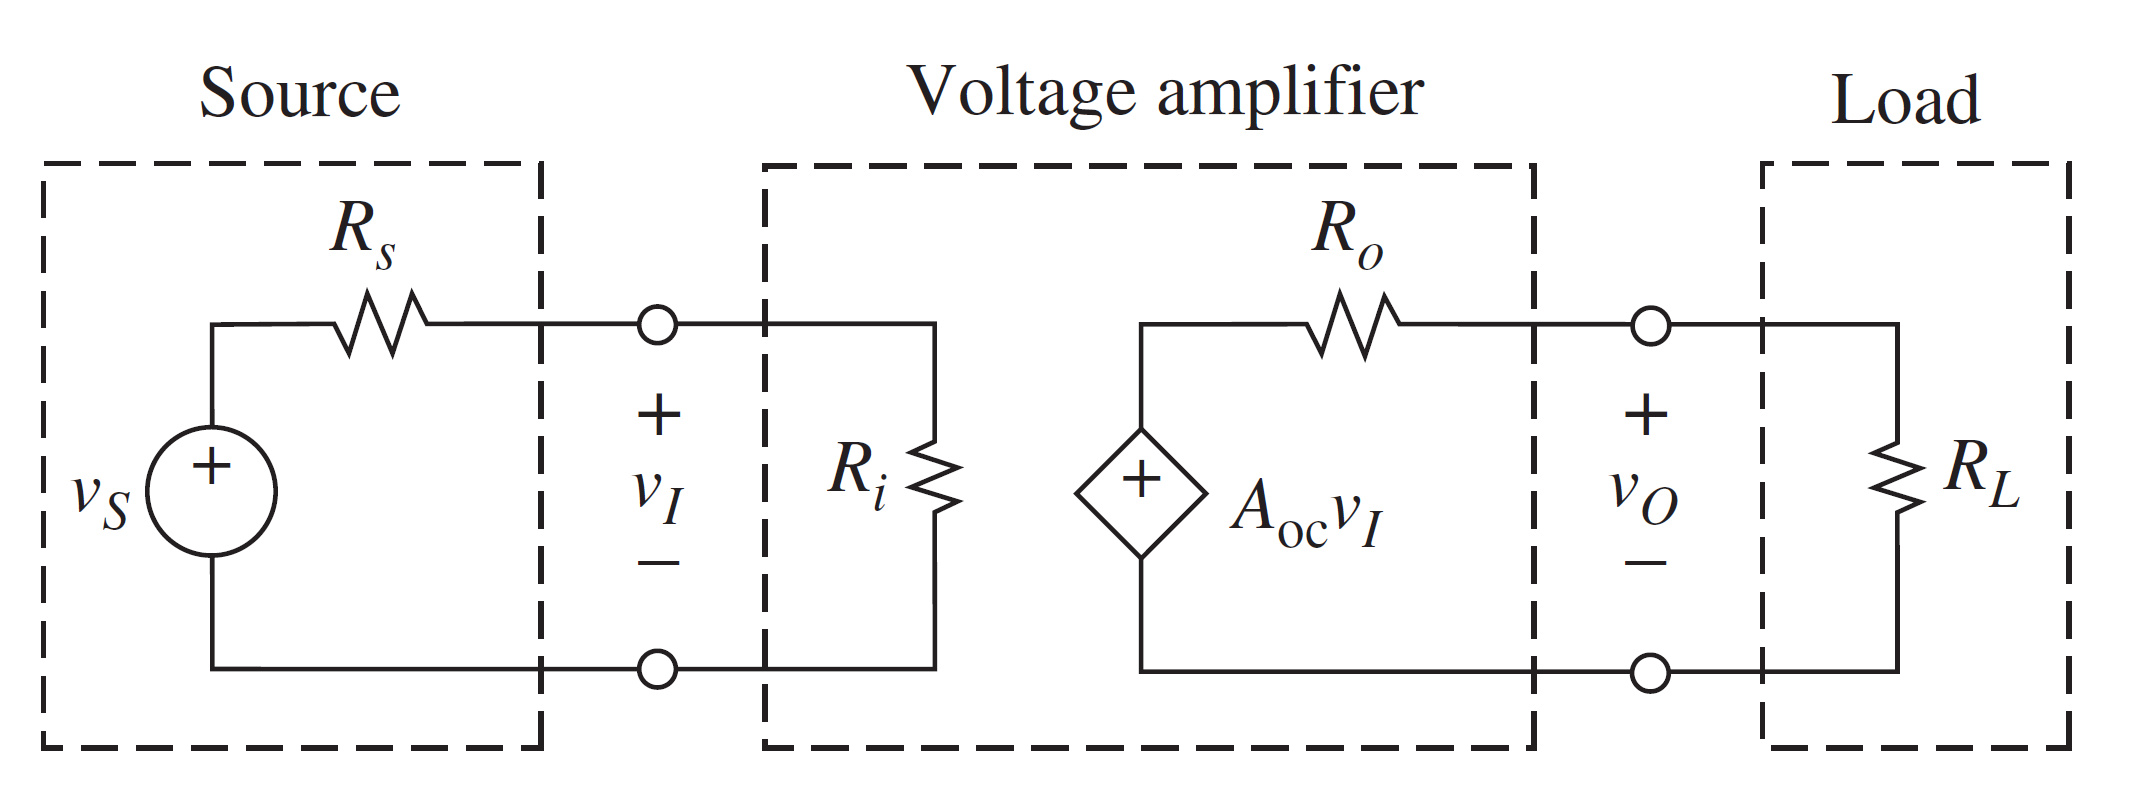
\includegraphics[scale=0.35]{1.1-Cuadrivector.png}
\caption{cuadrivector de un amplificador cualquiera con equivalentes Thevenin.}
\label{Fig:1.1-Cuadrivector}
\end{figure}

Cuando expresamos el amplificador de esta forma solemos decir que lo expresamos como un \textit{cuadrivector}. En ese caso tenemos que la señal de entrada no es $V_S$, ya que se ve afectada por las resistencias, de tal modo que:

\begin{equation}
 V_I = \dfrac{R_i}{R_S + R_i} V_{in}= \dfrac{R_i}{R_S + R_i} V_{S}
\end{equation}
donde $R_S$ es la resistencia thevenin equivalente de la fuente y $R_i$ es la \textbf{resistencia de entrada} ($R_E$ en la figura). Esto también ocurre con el voltaje de salida $V_0$, que se ve afectado por la resistencia de salida de tal forma que:

\begin{equation}
V_{out} \equiv V_O = \dfrac{R_L}{R_0 + R_L} A_V V_I
\end{equation}
siendo $A_V := A_{oc}$s la ganancia lineal de nuestro amplificador, $R_O$ la \textbf{resistencia de salida}, y $R_L$ el equivalente thevenin de la carga. Entonces la \textbf{ganancia de la fuente de carga} vendrá dada por:

\begin{equation}
\dfrac{V_O}{V_S} = \dfrac{V_{out}}{V_{in}} = \dfrac{R_{i}}{R_S + R_i} \dfrac{R_L}{R_O + R_L} A_V
\end{equation}

Antes de seguir debemos comprender algo fundamental. Estas resistencias no son resistencias reales, no son resistencias tangibles que tu puedas poner o medir en el circuito. Estas resistencias son simples conceptos matemáticos que nos ayudan a describir el circuito. Aunque incluso puedas pensar que se encuentran dentro de la caja negra del amplificador, en realidad no, no son reales, son \textbf{parámetros caracterizadores} del circuito, de tal forma que podamos relacionarlos con resistencias reales, ayudándonos a describir y entender mejor el circuito. \\

Por ejemplo: ¿Si la \textit{resistencia de entrada tiende a infinito} que ocurre? Pues que la señal de las fuentes es exactamente igual que la señal que llega al amplificador, además de que la intensidad que circula por la resistencia es nula. ¿Y si la \textit{resistencia de salida es nula}? En ese caso tendremos que la señal de salida $V_O$ depende únicamente de la señal amplificada y no de las cargas (resistencias) o la forma del circuito posterior. Como podemos ver realmente estas resistencias pueden ayudarnos a describir, a \textit{caracterizar}, el circuito. \\

De hecho a un amplificador que cumple estas condiciones (resistencia de entrada infinita y resistencia de salida nula) se le conoce como \textbf{amplificador operacional ideal}, ya que es el único amplificador que cumple que la ganancia del de fuente de carga depende exclusivamente de $A_V$: 

\begin{equation}
\dfrac{V_{out}}{V_{in}} = A_V
\end{equation}
donde esta ganancia será infinita, como veremos mas adelante. Para calcular las resistencias de entrada y salida echamos manos de las siguientes ecuaciones:

\begin{equation}
R_i = \dfrac{V_{in}}{I_{in}} \tquad R_O = \left. \dfrac{V_O}{I_O} \right|_{V_{in}=0}
\end{equation}

En escasas palabras: la resistencia de entrada es la relación entre intensidad y voltaje que hay en la fuente de entrada; y la resistencia de salida la relación entre intensidad y voltaje que hay en la resistencia de salida cuando \textit{las demás fuentes de tensión (independientes) son nulas}. Si no se ha entendido nada no o es preocupéis, estudiad los primeros ejemplos que hagamos (apartado \ref{Subsec:1.3}).



\subsubsection{Clasificación de los amplificadores}

Como ya hemos dicho un amplificador transforma una señal eléctrica en otra, pudiendo ser esta un voltaje (la más común) o intensidad. Entonces tendremos 4 tipos de amplificadores en función de cual es la señal de entrada y cual es la señal de salida, de tal modo que:


\begin{itemize}
\item \textbf{Amplificador de tensión:} le llega una señal de entrada de tensión y la transforma en otra de tensión.
\item \textbf{Amplificador de corriente:} le llega una señal de entrada de intensidad y la transforma en otra de intensidad.
\item \textbf{Amplificador de trans-conductancia:} le llega una señal de entrada de tensión y la  transforma en otra de intensidad.
\item \textbf{Amplificador de transresistencia:} le llega una señal de entrada de intensidad y la transforma en otra de tensión.
\end{itemize}


\begin{figure}[h!] \centering
\includegraphics[scale=0.70]{1.1-Clasificación.png}
\caption{a) Amplificador de tensión. b) Amplificador de tras-conductancia. c) Amplificador de corriente. d) Amplificador de transresistencia.}
\label{Fig:1.1-Clasificaion}
\end{figure}

Como podemos intuir ahora los equivalentes Thevenin se convierten en equivalentes Norton. Sabiendo esto podemos estudiar cual será las diferentes relaciones entre resistencias e intensidades. Véase la figura \ref{Fig:1.1-Clasificaion}.

\subsubsection{Saturación}

En general los amplificadores tienen una potencia (intensidad) máxima que pueden amplificar. A esta se le llama tensión de saturación. Si el amplificador es lineal tendremos una curva de amplificación como la de la figura \ref{Fig:1.1-Saturacion}. \\


La saturación cobra vital importancia en el marco práctico y experimental del estudio de amplificadores. Obviamente la energía no se crea de la nada, por lo que la señal de salida estará limitada por lo que podamos aportar externamente sin ser una señal de entrada. Es decir, depende del voltaje que le suministremos al amplificador. En el siguiente tema lo entenderemos mejor. Consecuentemente conocer cual es la señal de entrada máxima a partir del cual la salida entra en saturación es sumamente importante en este temario.

\begin{figure}[h!] \centering
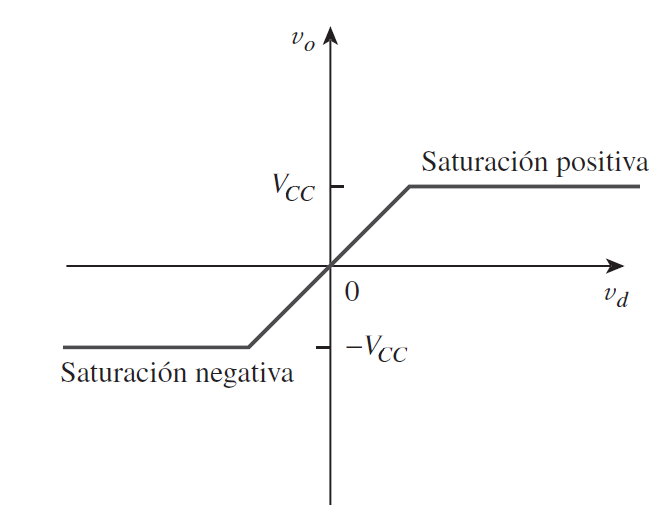
\includegraphics[scale=0.5]{0.Saturacion}
\caption{saturación para un amplificador lineal. $V_d$ es la señal de entrada.}
\label{Fig:1.1-Saturacion}
\end{figure}




\subsection{Amplificador operacional}

Un amplificador operacional se representa con un triángulo, con na entrada inversora, una entrada no inversora (son simples nombres, con una razón de ser que mas adelante se entenderá), una salida y un suministro externo (figura \ref{Fig:1.2-Amplificador}). \\


\begin{figure}[h!] \centering
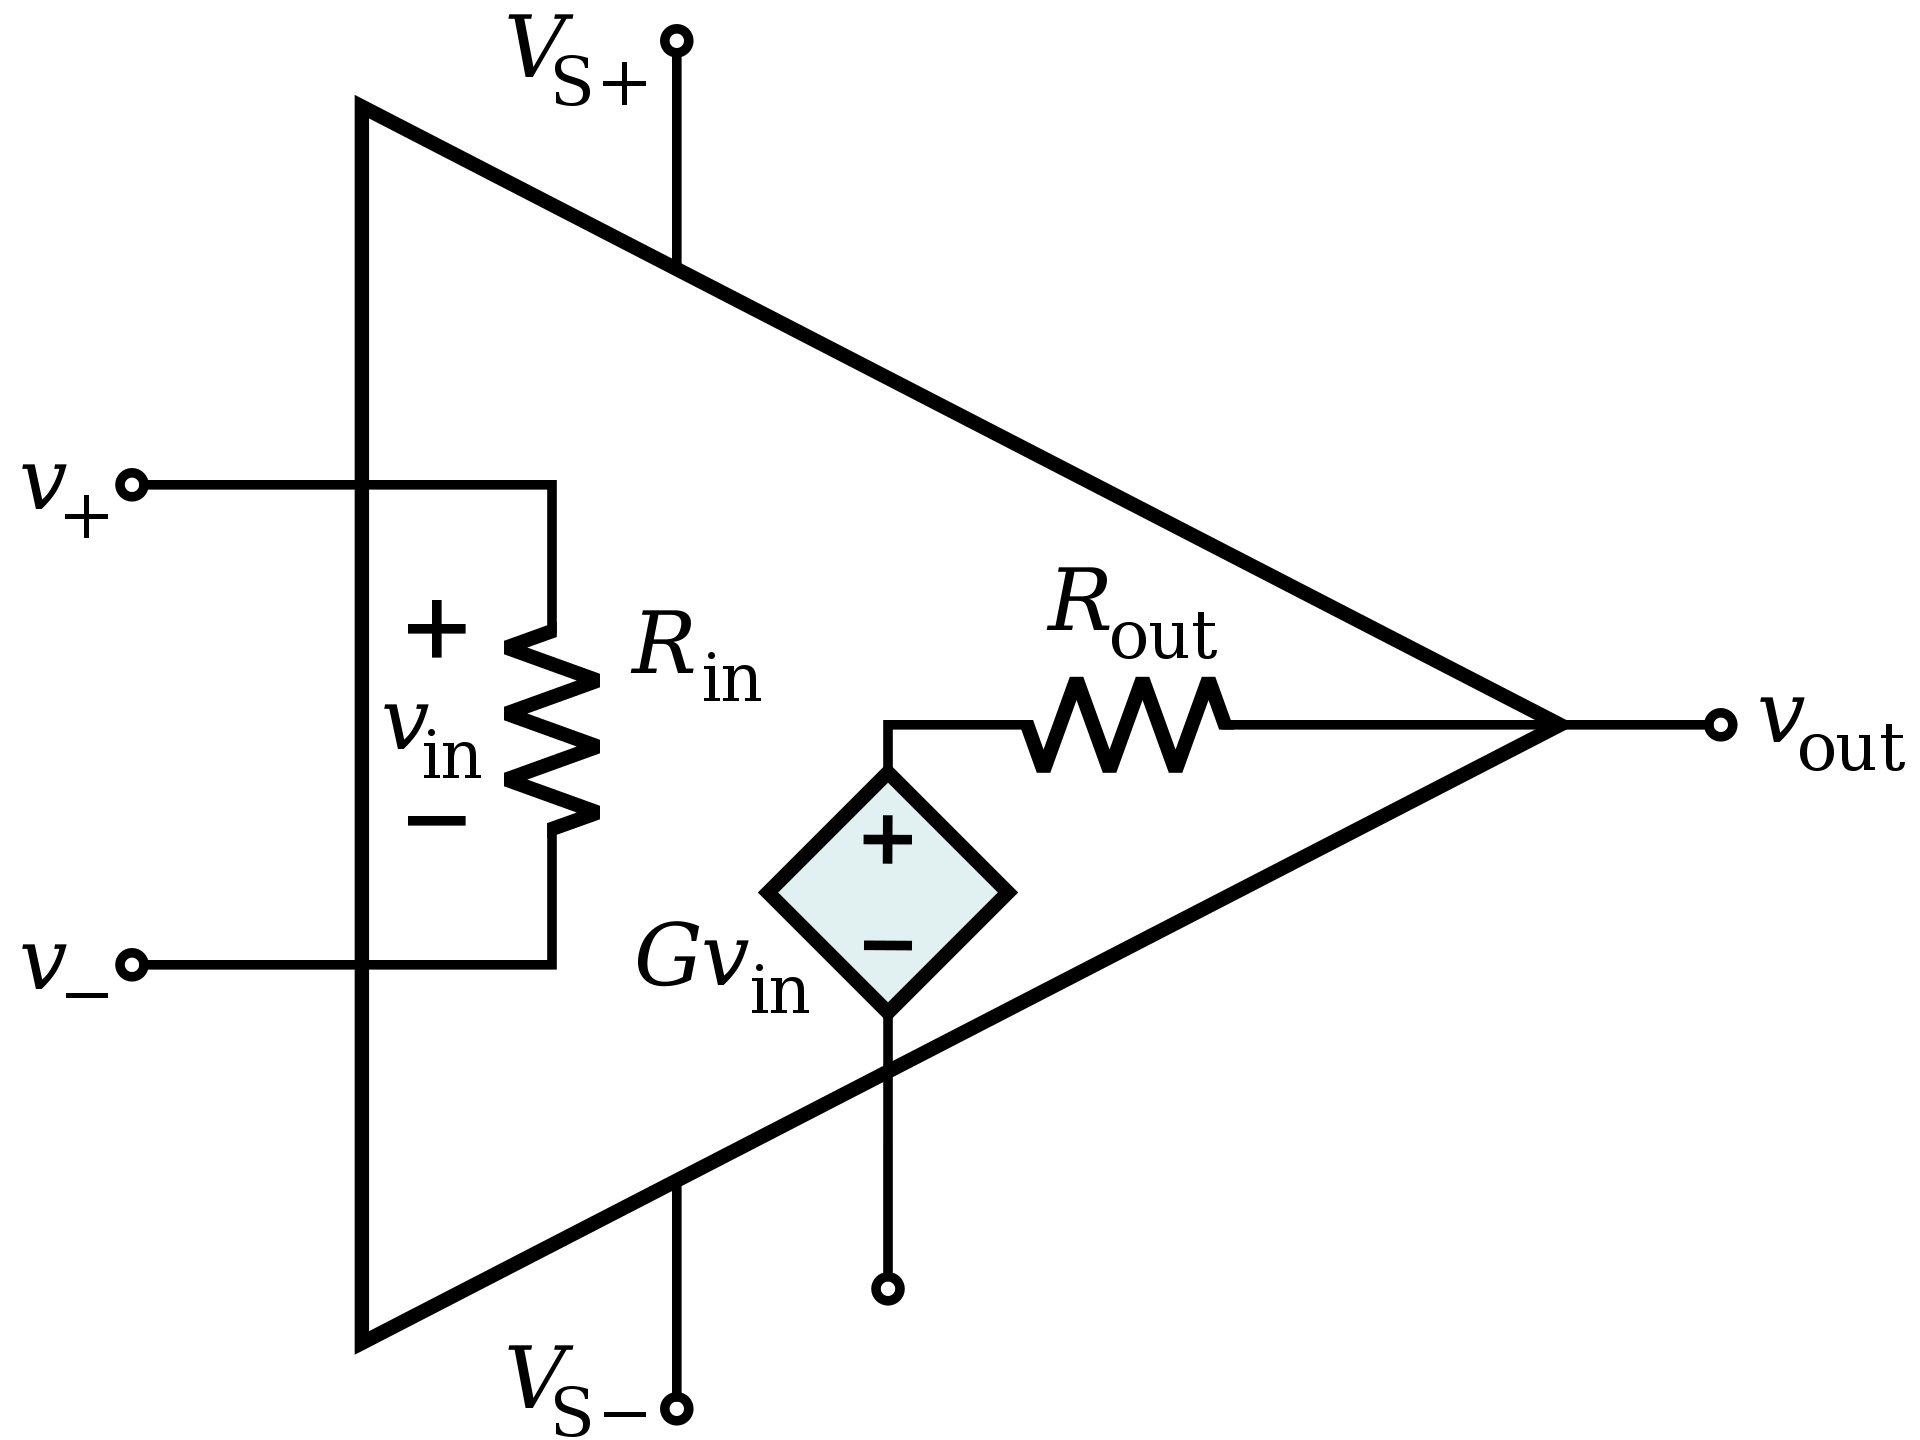
\includegraphics[scale=0.10]{1.2-Amplificador.png}
\caption{amplificador operacional}
\label{Fig:1.2-Amplificador}
\end{figure}

En general veremos como la señal de entrada $-$ se encuentra en la parte superior y $+$ en la parte de abajo (posiciones intercambiadas). Como podemos ver presenta los mismos elementos que el cuadrivector. Por si no queda claro, todo voltaje está unido a una tierra común, para evitar cargas flotantes (diferencias de potencial aplicadas respecto a otros voltajes). Para minimizar el hacinamiento en los diagramas de circuitos es común no mostrar las conexiones de energía. A la diferencia

\begin{equation}
V_i = V_+ - V_-
\end{equation}
se le llama \textbf{voltaje diferencial de entrada}. Estudiemos ahora el \textit{amplificador operacional ideal}, con las características ya mencionadas.

\subsubsection{Amplificador operacional ideal}
El amplificador operacional ideal es la imagen a la que cualquier tipo de amplificador operacional real trata de asemejarse. Además de esto puede servir como aproximación que puede predecir con cierta exactitud los valores reales, por lo que su estudio es fundamental para poder predecir el comportamiento de un amplificador operacional real. \\

El amplificador operacional ideal va ligado al efecto de conseguir ganancia infinita de potencia lo que implica no absorber potencia en la entrada y proporcionar toda la potencia que se pida en la salida. Para lo primero necesitamos que la resistencia de entrada se haga infinita para amplificadores de tensión y nula para amplificadores de corriente. Lo segundo se logra haciendo que toda la potencia de la fuente del equivalente de salida se desarrolle sobre la carga $R_L$, lo que se alcanza haciendo nula la resistencia de salida (salida de tensión) o infinita (salida de corriente). \\

Entonces definimos un \textbf{amplificador operacional ideal} como aquel amplificador que verifica que:

\begin{itemize}
\item Ganancia de tensión infinita. Esto nos lleva a que si la tensión de salida es finita, la entrada de tensión sea nula ($V_i \rightarrow 0$).

$$ A_V \rightarrow \infty $$

\item Resistencia de entrada infinita. Lo que implica que el amplificador operacional no admite corriente por sus entradas.

$$ R_{in} \rightarrow \infty $$
que se suele representar como un circuito abierto. Esto lleva a que no circule intensidad entre los entradas.

\item Resistencia de salida nula. Con este supuesto, el dispositivo es capaz de mantener la tensión de salida sea cual sea la carga.

$$ R_{out} \rightarrow 0 $$
que se representa mediante un cortocitcuito (cable sin resistencia).


\end{itemize}

Es importante mencionar que como circuito activo que es el amplificador operacional \textit{necesita alimentación} para funcionar. La forma de analizar el circuito es bastante simple y se deriva de dos consideraciones que ya hemos mencionado:

\begin{itemize}
\item Por ninguna de las dos entradas circula corriente, ya que su resistencia de entrada es infinita. A este fenómeno se le llama \textbf{cortocircuito virtual}.
\item Si el dispositivo tiene tensión de salida finita y $A_d$ (ganancia) es infinita la única opción es que $v_d$ sea nula (diferencia de potencial de entrada).
\end{itemize}

\begin{figure}[h!] \centering
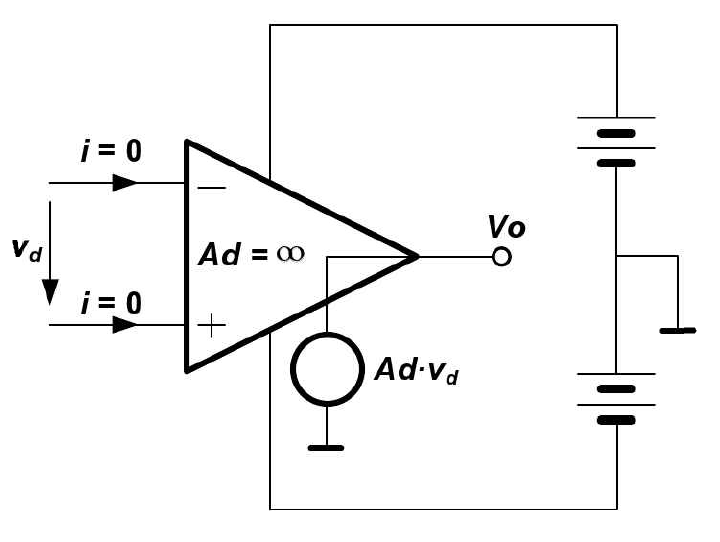
\includegraphics[scale=0.5]{1.1.Amplificador_ideal.png}
\end{figure}

Para solucionar cualquier ejercicio donde haya amplificadores operacionales ideales (A.O.I) será fundamental aplicar estas dos reglas. El resto del análisis se basará en hacer Kirchoff, equivalentes Thevenin y Norton y usar el principio de superposición.



\subsubsection{Lazo abierto y cerrado}

Decimos 	que un amplificador operacional está en \textbf{lazo abierto} cuando la salida del amplificador no se conecta directamente a su entrada inversora. Cuando si se conecta directamente a su entrada inversora decimos que el amplificador operacional esta en \textbf{lazo cerrado}. \\

En otras palabras, podemos decir que cuando un circuito esta en
 lazo abierto no se retroalimenta. Cuando está en lazo cerrado si se retroalimenta. Este concepto es sumamente importante posteriormente, conviene tenerlo muy claro. Decimos que se retroalimenta porque parte de la salida se conecta a la entrada. \\
  
 
Cuando un amplificador operacional está en lazo abierto la resistencia de entrada $R_i$ es infinita, y cuando está en lazo cerrado la resistencia de entrada es finita. 

\subsubsection{Retroalimentación positiva y negativa}


Como hemos dicho vamos a explicar que es la retroalimentación. La mayoría de los circuitos que estudiaremos en este tema poseen algún  tipo de retroalimentación (inversor...) por lo que es muy importante saber que es. \\

La estructura básica de un circuito de retroalimentación se incluye en la figura \ref{Fig:1.2.3-Retroalimentacion}. Como se puede ver las flechas indican el sentido de la señal, el símbolo genérico $x$ ya sea para una señal de voltaje o de corriente. 



\begin{figure}[h!] \centering
\includegraphics[scale=0.5]{1.2-Retroalimentación.png}
\caption{}
\label{Fig:1.2.3-Retroalimentacion}
\end{figure}


Como podemos ver en la estructura hay varios elementos: la fuente envía señal al amplificador (triángulo) que posee una ganancia lineal $a$. Luego existe una estructura que relaciona el voltaje de salida con el voltaje de entrada y está dominado por un $\beta$. Con mas claridad distinguimos los siguientes bloques:



\begin{itemize}
\item Un \textit{amplificador} que acepta una señal de entrada $x_d$ que se ve afectada por la $x_i$ y por la retroalimentación $x_f$; produciendo una señal de salida:

\begin{equation}
x_0 = a x_d
\end{equation}
donde $a$ es la ganancia de ciclo abierto (lazo abierto).

\item Una \textit{malla de retroalimentación} por la que entra $x_0$ y produce una \textit{señal de retroalimentación}

\begin{equation}
x_f = \beta x_0
\end{equation}
donde $\beta$ es el \textit{factor de retroalimentación}.

\item Una \textit{malla sumadora} ($\Sigma$) es el dispositivo que suma $x_i$ y $x_f$ para generar $x_d$: 

\begin{equation}
x_d = x_i - x_f
\end{equation}
que es la que decide si la retroalimentación es negativa o positiva. La \textbf{retroalimentación negativa} surge del ehecho de que se está \textit{alimentando} una porción de $x_0$ de regreso a la entrada donde \textit{resta} de $x_i$ para producir la señal reducida $x_d$. Podría sesr positiva si se sumara.
\end{itemize}

Como podemos ver esto será el \textit{el esquema mas general}, y que en realidad será completamente análogo a un amplificador operacional donde la ganancia vendrá dada por:

\begin{equation}
A = \dfrac{a}{1+ a \beta}
\end{equation}
que se llama \textbf{ganancia de lazo cerrado}. La retroalimentación negativa implica que $a \beta$  es positivo y por lo tanto $A<a$. Esta relación del divisor la llamamos \textbf{cantidad de retroalimentación}. Al producto $a\beta$ lo llamamos \textbf{ganancia de lazo} y lo describimos como

\begin{equation}
T \equiv a \beta
\end{equation}

De hecho podemos estudiar un amplificador operacional ideal así. Si la ganancia de nuestro amplificador operacional $a \rightarrow \infty$ tendríamos que la amplificación será:

\begin{equation}
A_{\mathrm{ideal}} = \lim_{a \rightarrow \infty} A = \dfrac{1}{\beta}
\end{equation}
por lo que $A$ se vuelve indepiente de $a$ y solo depende de la malla de retroalimentación. Es decir que el inverso del factor de retroalimentación de un circuito será exactamente igual que la ganancia para dicho circuito amplificador si suponemos que sus amplificadores operacionales son ideales. Dicho de otro modo, podemos expresar la \textit{ganancia de lazo cerrado} como:

\begin{equation}
A = \dfrac{A_{\mathrm{ideal}}}{1+1/a\beta}
\end{equation}


\subsection{Configuraciones básicas del amplificador \label{Subsec:1.3}} 

Cuando conectamos componentes externos alrededor de un amplificador operacional obtenemos lo que se llama \textit{circuito amplificador operacional}. Es crucial que se entienda la diferencia entre estos un circuito y un amplificador operacional individual: este último es un componente del primero. Aunque pueda entenderse un circuito como un amplificador operacional individual donde los componentes externos forman parte de la ganancia no hay que confundirlo. \\

Vamos a analizar cada circuito para el caso real y para el caso ideal, para ver las diferencias y para luego poder entender mejor que es la retroalimentación, el comportamiento mas general de un amplificador operacional...

\subsubsection{Amplificador no inversor}

\begin{figure}[h!] \centering
\includegraphics[scale=0.25]{1.3-Amplificador-inversor.png}
\caption{amplificador no inversor.}
\label{Fig:1.3-Amplificador-inversor}
\end{figure}


\begin{figure}[h!] \centering
\includegraphics[scale=0.3]{1.3-Amplificador-inversor-2.png}
\caption{amplificador no inversor (feedback network = malla de retroalimentación).}
\label{Fig:1.3-Amplificador-inversor-2}
\end{figure}


Sea el circuito de la figura \ref{Fig:1.3-Amplificador-inversor} y \ref{Fig:1.3-Amplificador-inversor-2}. Tendremos que tenemos que calcular la relación entre la señal de salida $V_O$ y la señal de entrada $V_i$. Analicemos el amplificador como si fuera un amplificador operacional real. En ese caso tendremos que tener en cuenta todos los efectos posibles. \\

Como se puede ver existen dos conexiones que afectal al valor de $V_O$: el voltaje que se genera por el amplificador y el voltaje que se genera por la malla de retroalimentación. Tendremos entonces que calcular esta por separado. Tenemos que analizar por kirchoff todo el circuito. \\

Para estudiar la malla de retroalimentación calculamos el valor de $V_O$ en función de $V_N$ de tal modo que aplicando la fórmula de división de voltaje, o resolviendo el análisis de la figura \ref{Fig:1.3-Amplificador-inversor-3}. En ese caso podemos ver claramente que la relación es:

\begin{equation}
V_N = \dfrac{1}{1+R_2/R_1} V_O
\end{equation}
el voltaje $V_N$ representa la fracción de $V_O$ que retroalimenta a la entrada iinversora. En consecuencia, la función de la malla resistiva es crear \textit{retroalimentación negativa} alrededor del amplificador operacional. \\


\begin{figure}[h!] \centering
\includegraphics[scale=0.35]{1.3-Amplificador-inversor-3.png}
\caption{}
\label{Fig:1.3-Amplificador-inversor-3}
\end{figure} 


Es entonces claro que $V_O$ viene dado por $aV_D$, por lo que tendremos que igualar $V_0 = a V_D = a (V_P - V_N)$. En ese caso como $V_P = V_I$ tendremos que desarrollando todo:

\begin{equation}
V_O = a \parentesis{V_I - \dfrac{1}{1+R_2/R_1} V_O} 
\end{equation} 
de tal modo que si despejamos obtendremos el real de la amplificación en ganancia del voltaje del circuito de amplificación operacional, de tal modo que:

\begin{equation}
A = \dfrac{V_O}{V_I} = \dfrac{1+R_2/R_1}{1+(1+R_2/R_1)/a}
\end{equation}

Como $A$ es positivo tenemos que la polaridad de $V_O$ es exactamente la misma que la de $V_I$ (si un voltaje es negativo el otro será negativo también). De aquí el nombre de \textit{amplificador no inversor}. Podemos considerar perfectamente el circuito amplificador operacional como un amplificador operacional con ganancia $A$ y obtendríamos exactamente el mismo resultado. Es una frase: \textit{el circuito amplificador operacional es en sí mismo un amplificador}. \\

%La ganancia $A$ del circuito amplificador operacional y la ganancia del amplificador operacional $a$ son muy diferentes, lo cual no es sorprendente, ya que ambos comparten la misma salida y diferente entradas ($V_I$ para el primero y $V_D$ para el segundo). Para recalcar esta diferencia llamamos a $a$ la \textbf{ganancia en lazo abierto} y a $A$ la \textbf{ganancia en lazo cerrado}. \\

%¿Por qué escribimos estos nombres? Podemos ver que la ganancia $a$ es la ganancia que tendría el circuito en el caso de que no existiera malla de retroalimentación. En general cuando no hay retroalimentación decimos que el sistema está en lazo abierto. Dado que $A$ es la ganancia cuando esta en lazo cerrado (hay retroalimentación) tiene ese nombre. \\



Si estudiamos el caso para un amplificador ideal lo único que tenemos que estudiar es que $a \rightarrow \infty$. En ese caso es obvio que:

\begin{equation}
A_{ideal} = \lim_{a \rightarrow \infty} A = 1 + \dfrac{R_2}{R_1}
\end{equation}
si lo estudiamos por un análisis de circuitos normal suponiendo que la $V_D = 0$ (otra de las condiciones) llegaremos al resultado final. Instamos al lector a comprobar esta relación. Habiendo hecha la anterior esta resultará mucho mas sencilla. Podemos calcular las resistencias de entrada y resistencias de salida para el amplificador inversor (ideal) con las ecuaciones que hemos dado: \\

\begin{equation}
R_i = \infty \tquad R_O = 0
\end{equation}


%En este límite $A$ se vuelve independiente de $a$ y su valor lo establece de manera exclusiva la razón de las resistencias externas. Ahora se puede apreciar la razón por la que se deseaba que un amplificador operacional fuera lo mas parecido al ideal. Así un circuito cuya ganancia de lazo cerrado dependa sólo de una razón de resistencias, ofrece muchas ventajas para el diseñador, ya que hace más fácil adaptar la ganancia a la aplicación en cuestión. ¿Quieres un amplificador con ganancia variable? Entonces haga variable $R_1$ o $R_2$ por medio de un potenciometro. ¿Quieres una ganancia de $2 V/V$? Tenemos que $R_2/R_1=1$. \\

%Otra ventaja es que la ganancia $A$ puede hacerse tan exacta y estable como se quiera. Incluso puede eliminarse la dependencia de factores como la temperatura: si queremos una ganancia concreta solo es necesario que se rastreen una a la otra con la temperatura de modo que mantengan una razón constante. Incluso si las resistencias tienen mala calidad, siempre que la razon entre estas sea la deseada obtendremos la amplificación querida. Comparar esto con el hecho de que la ganancia $a$ dependa de resistores, diodos, transistores dentro del amplificador operacional convierte a la electrónica en una rama maravillosa: podemos crear un circuito con un alto rendimiento con el uso de componentes deficientes. \\

%Como se ha demostrado el circuito amp. op. es en si mismo un amplificador, por lo que también presenta resistencias de entrada y de salida. Ahora podemos ver mas que nunca que son parámetros caracterizadores: no existen pero podemos calcularlos, para así expresar el circuito como un cuadrivector con un análisis mucho mas directo. A la resistencia de entrada $R_i$ también se le conoce como \textbf{resistencia de entrada de lazo cerrado} y a la resistencia de salida $R_o$ como \textbf{resistencia de salida de lazo cerrado}. \\

%Como ya hemos dicho podemos calcular el valor de estas. Aunque se hablará en la siguiente sección mas de estos parámetros podemos adelantar un poco cual es su significado físico. El valor de $R_i$ nos da una medida de cual es la intensidad que circula entre los puntos $V_I$. Si por ejemplo $R_i \rightarrow \infty$ tendríamos que la intensidad sería cero. De ser $R_i = 0$ tendríamos que esta sería infinita, además de lo que ya dijimos (señal de entrada depende únicamente de $V_S$). Si la señal de entrada al amplificador operacional no es $V_S$ básicamente $R_i \neq \infty$. El valor de $R_o$ básicamente nos dice cual es la dependencia de la resistencia de salida $R_L$. \\

%Para un amplificador operacional inversor ideal tendremos que $R_i = \infty$ y que $R_o = 0$. Lo primero es obvio, ya que por la fuente de tensión $V_I$ no circula intensidad, ya que la resistencia de entrada del amplificador operacional ideal es infinita. 

\subsubsection{Buffer}

El amplificador buffer o \textit{seguidor de voltaje} es un circuito amplificador que deja la ganancia exactamente en uno (sin cambios de polaridad). Por eso mismo también se le llama \textit{seguidor de voltaje}. En el caso de que el amplificador operacional sea idea podemos construirlo fácilmente una vez hemos visto el amplificador no inversor, ya que queremos que $R_2/R_1 \rightarrow 0$. Para esto hacemos que $R_2 \rightarrow 0, R_1 \rightarrow \infty$. Entonces el circuito nos quedaría algo como la figura \ref{Fig:1.3-Buffer}. \\



\begin{figure}[t] \centering
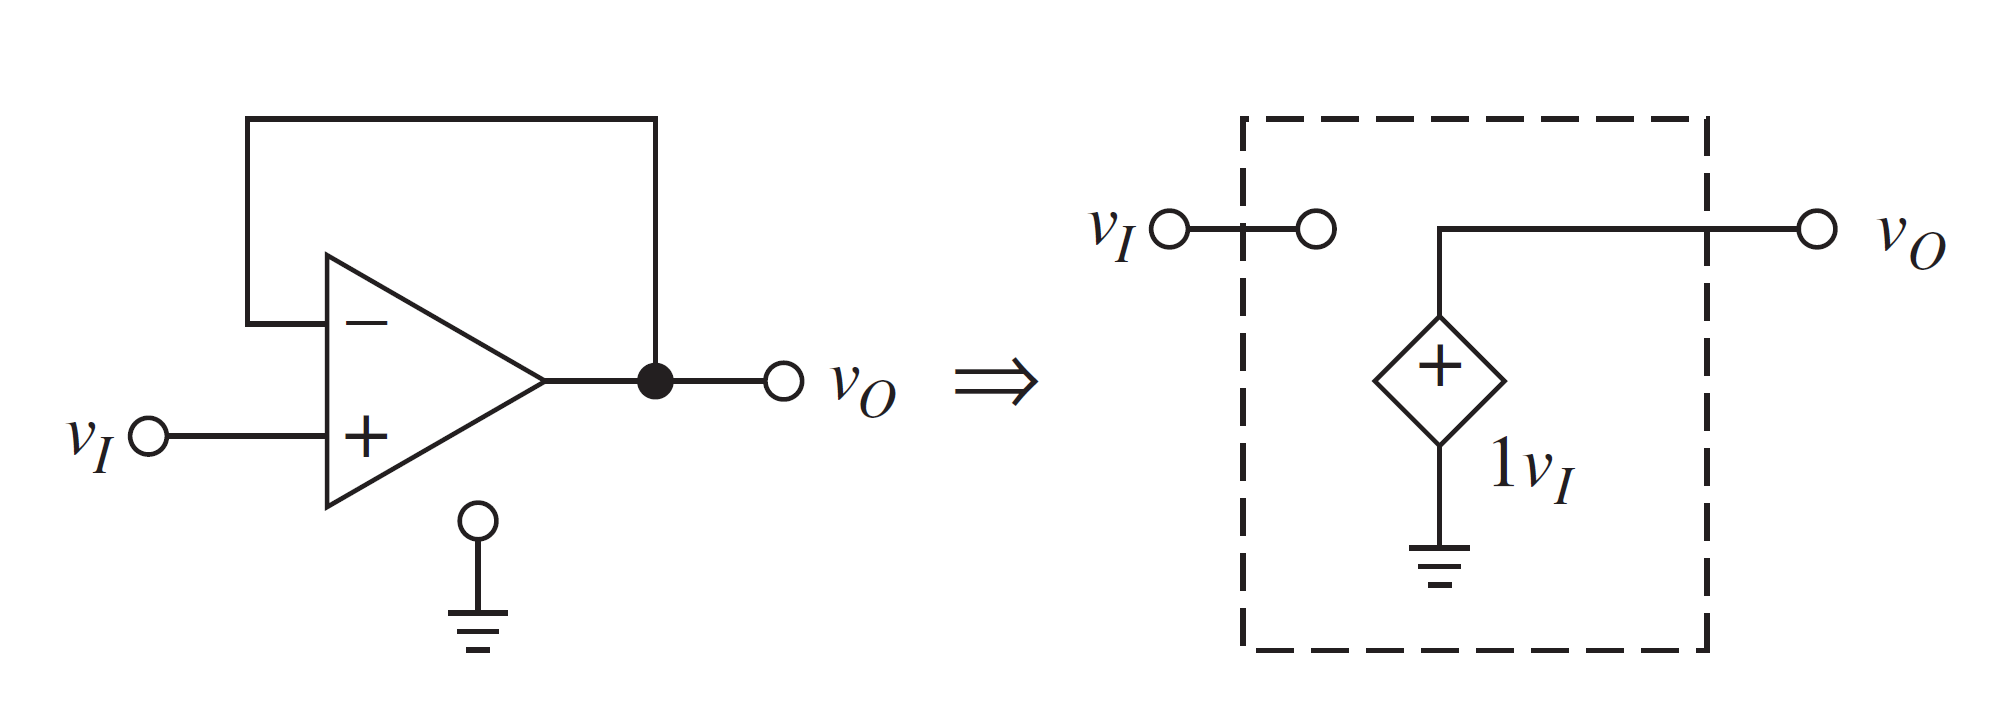
\includegraphics[scale=0.4]{1.3-Buffer.png}
\caption{seguidor de voltaje y su circuito equivalente ideal.}
\label{Fig:1.3-Buffer}
\end{figure} 

Uno puede preguntarse el porque crear un buffer con ganancia uno, ya que simplemente conectar los cables entre los voltajes haría exactamente lo mismo. Véase figura \ref{Fig:1.3-Buffer-1}. Y en efecto esto sería cierto \textit{si las fuentes fueran ideales}. Sin embargo las fuentes no son nunca ideales, siempre tienen una resistencia asociada, por lo que conectándolos de manera directa tendremos que $V_S > V_L$. Si pusieramos un buffer ideal ignoraríamos estas resistencias asociadas a las fuentes ($R_S,R_L$) ya que la ganancia $R_i = 0$ implica que no hay intensidad circulando por $R_S$ y $V_I = V_S$. Y como $R_O = \infty$ tendríamos que ignoramos $R_L$.  \\


\begin{figure}[t] \centering
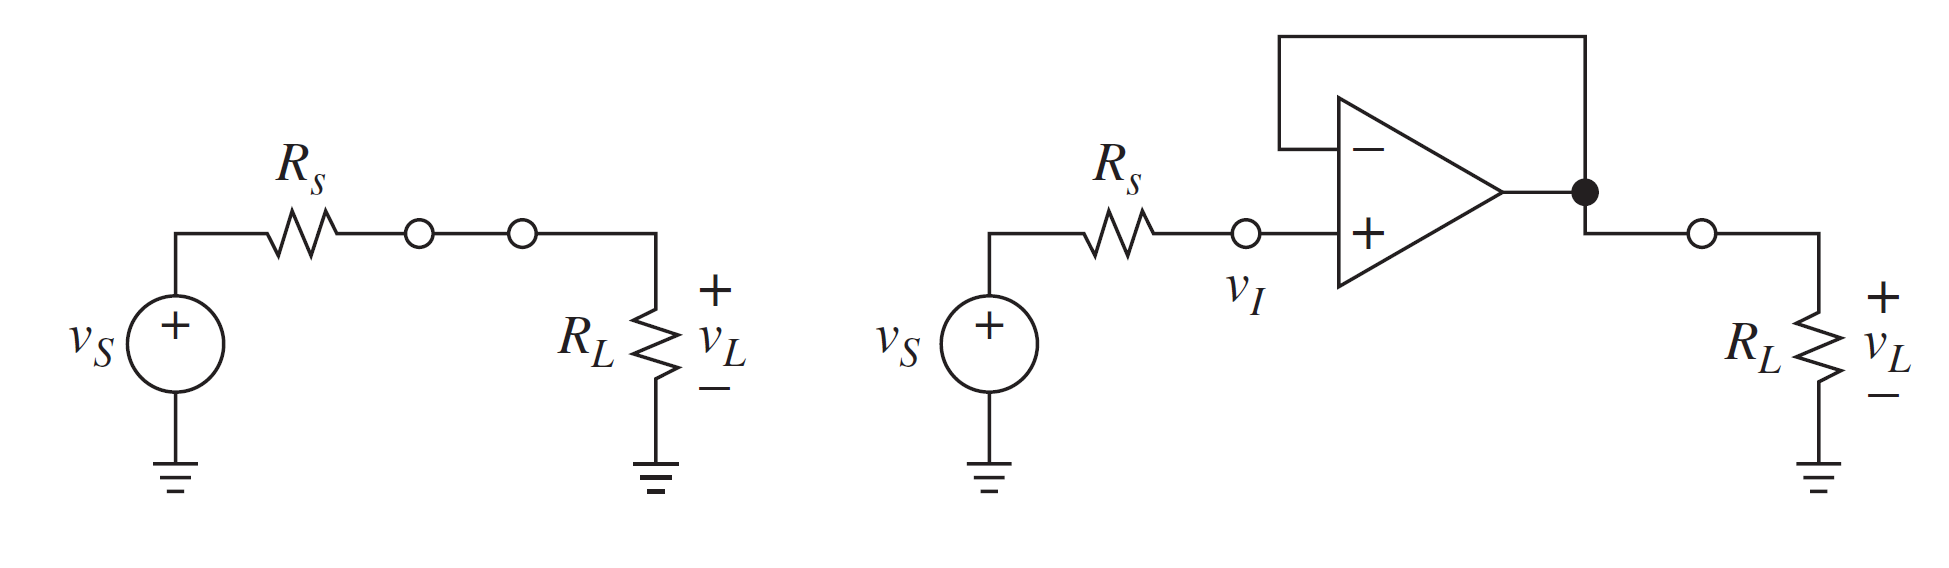
\includegraphics[scale=0.4]{1.3-Buffer-1.png}
\caption{}
\label{Fig:1.3-Buffer-1}
\end{figure} 


\subsubsection{Amplificador inversor}



El amplificador inversor es un circuito amplificador inversor como el que podemos ver en la figura \ref{Fig:1.4-Amplificador-Inversor}. Está claro que $V_O = a V_D$, y que $V_D = V_N$. Entonces tenemos que hallar $V_N$ en función de $V_I$ y $V_O$. Podemos estudiar por superposición el fenómeno, de tal manera que:

\begin{equation}
V_N = \left. V_N \right|_{V_O=0} +   \left. V_N \right|_{V_I=0}
\end{equation}
Que lleva (tal y como hemos hecho para el amplifcador inversor) a que:

\begin{equation}
V_N = \dfrac{1}{1+R_1/R_2} V_I + \dfrac{1}{1+R_2/R_1} V_O 
\end{equation}
Finalmente obtendremos que despejando $V_O = -  a V_N$ que:

\begin{equation}
A = \dfrac{V_O}{V_I} = \dfrac{-(R_2/R_1)}{(1+(1+R_2/R_1)/a)}
\end{equation}
Se puede ver claramente que la amplificación en este caso conlleva un cambio de polaridad  respecto $V_I$. Por eso mismo lo llamamos amplificador inversor. Ahora si estudiamos el amplificador operacional inversor ideal tendremos que:

\begin{equation}
A_{\mathrm{ideal}} = \lim_{a \rightarrow \infty} A = - \dfrac{R_2}{R_1}
\end{equation}

En ese caso la ganancia de lazo cerrad solo depende de resistencias externas lo que brinda las ventajas mencionadas para el amplificador no inversor: ganancia variable, con un valor estable y capaz de eliminar deficiencias de los elementos.  \\

Si tratamos de calcular las resistencais de entrada y de salida de lazo cerrado ($R_i, R_o$) tendremos que el resultado llevará a que:

\begin{equation}
R_i = R_1 \tquad R_O = 0
\end{equation}




\begin{figure}[t] \centering
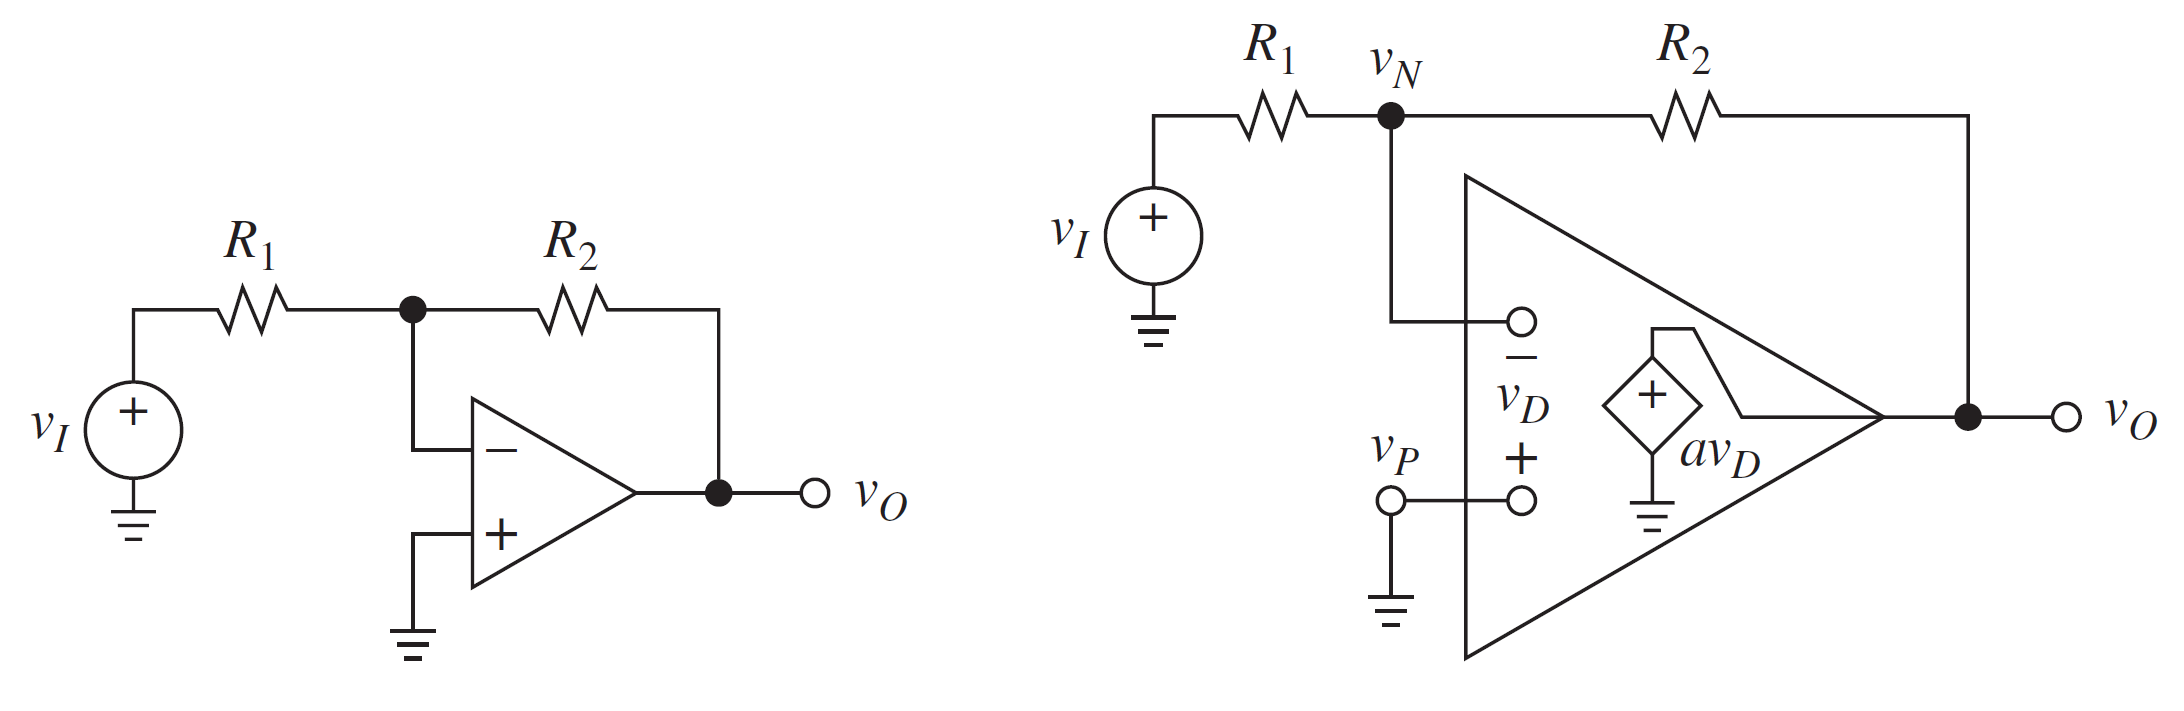
\includegraphics[scale=0.4]{1.4-Amplificador-inversor.png}
\caption{amplificador inversor.}
\label{Fig:1.4-Amplificador-Inversor}
\end{figure} 


\subsubsection{Amplificador sumador}

El amplificador sumador consta de un amplificador operacional y un circuito como el de la figura \ref{Fig:1.3.5.-Amplificador-Sumador}. Como podemos ver tiene varias entradas de potencial, en la figura 3, pero puede generalizarse para un numero arbitrario de ellas.\\

Como podemos ver tiene la forma de un amplificador inversor pero con varias entradas. Por el uso de la ley de Ohm podemos ver que en el caso de que sean amplificadores ideales tendremos que:

\begin{equation}
\dfrac{V_1}{R_1}+\dfrac{V_2}{R_2}+\dfrac{V_3}{R_3}=-\dfrac{V_0}{R_F}; \tquad V_0 = - \parentesis{\dfrac{R_F}{R_1}V_1+\dfrac{R_F}{R_1}V_1+\dfrac{R_F}{R_1}V_1}
\end{equation}

Dado que es la superposicion de amplificadores operacionales inversos podemos intuir cuales son las resistencias de entrada y salida. De no darse cuenta podemos usar las ecuaciones ya mencionadas. Los resultados serán:

\begin{equation}
R_{ik} = R_k \quad k =1,2,3 \tquad R_O=0
\end{equation}
Si las tres resistencias son iguales la ecuación lleva a que el voltaje final es proporcional a suma de voltajes.



\begin{figure}[h!] \centering
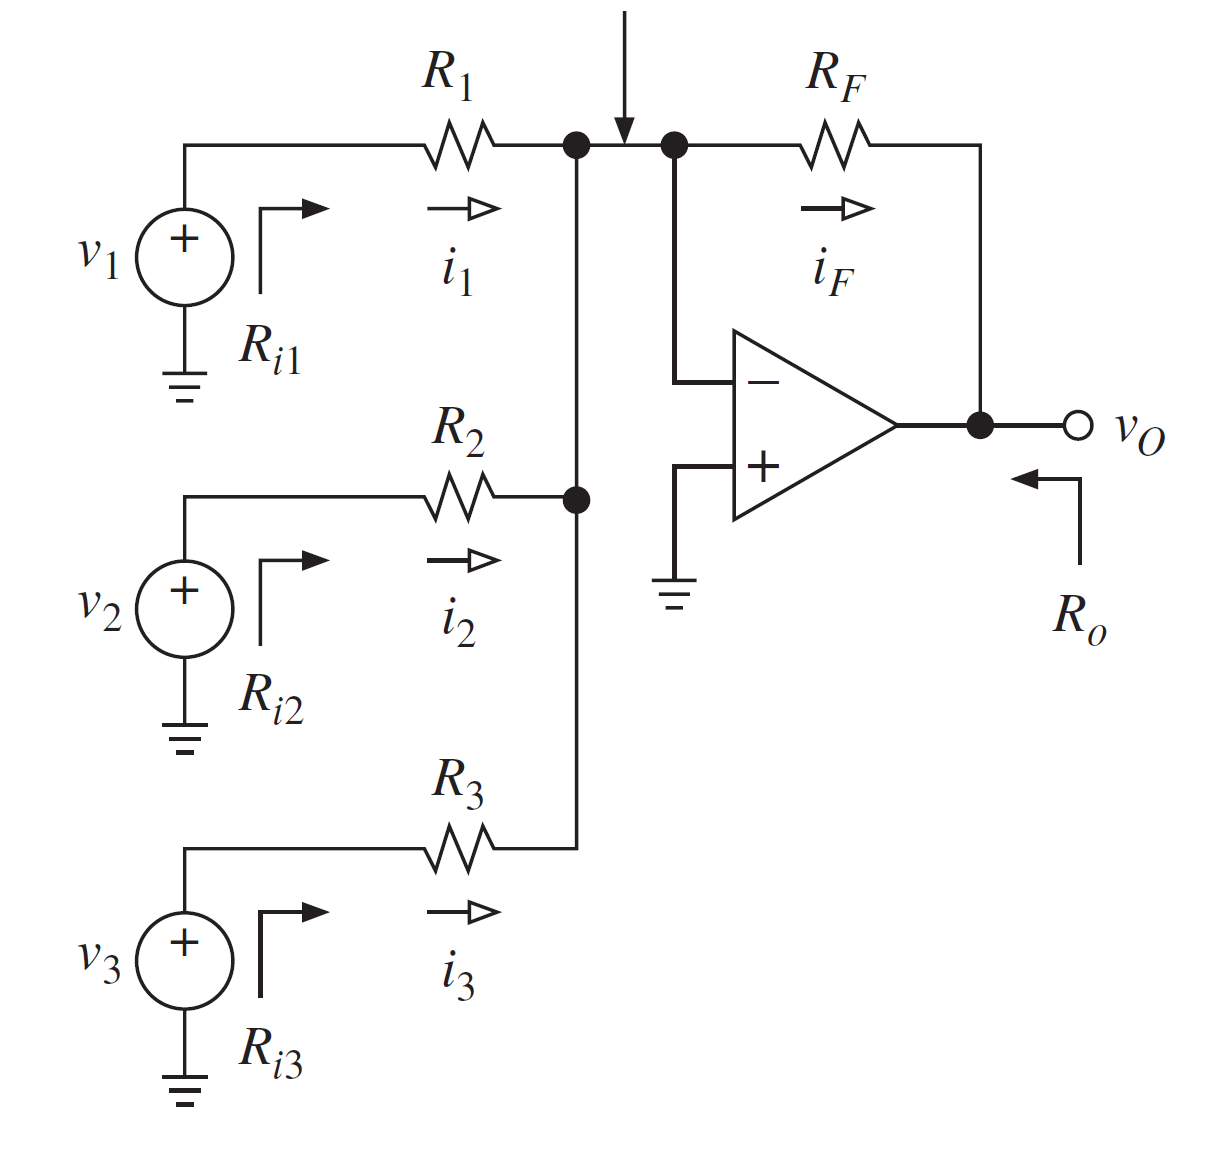
\includegraphics[scale=0.4]{1.5-Amplificador-sumador.png}
\caption{amplificador sumador.}
\label{Fig:1.3.5.-Amplificador-Sumador}
\end{figure} 

\subsubsection{Amplificador derivador}
El amplificador derivador (igual que el integrador) son circuitos que usan condensadores y por tanto que usan corriente alterna ($i(t),v(t)$) tal y como se puede ver en la figura \ref{Fig:1.3.6.-Amplificador-Derivador}. En todos los ejercicios anteriores hemos supuesto una corriente continua estable ya que el resultado será completamente análogo (si son ideales los amplificadores). Dado que $i_C=i_R$ tendremos que:

\begin{equation}
C \dfrac{\D v_I}{\D t} = \dfrac{1}{R}  v_O 
\end{equation}
o lo que es lo mismo:

\begin{equation}
v_O = RC \dfrac{\D v_I}{\D t}
\end{equation}
De ahí viene que se llame circuito derivador, ya que la salida será la derivada de la entrada. En el caso de que haya una corriente sinusoidal, usando la expresión compleja ($j \equiv $ desfase $\pi/2$) tendremos que:

\begin{equation}
v_O = jRC \omega  \cdot v_I  
\end{equation}


\subsubsection{Amplificador integrador}

Tenemos que el análisis del circuito (figura \ref{Fig:1.3.7-Amplificador-Integrador}) es exactamente igual que en el derivador. Como $i_R = i_C$ tendremos que $(v_I-0) / R = C  (0-\D v_O / \D t)$ de tal modo que al integrar respecto $t$ tenemos que:

\begin{equation}
v_O (t) = - \dfrac{1}{RC} \int_{0}^t v_I (t) \D t + v_O (0)
\end{equation}
donde $v_O (0)$ es el valor de la salida en $t=0$, aunque depende de la carga almacenada inicialmente en el condensador/capacitor. 


\begin{figure}[h!] \centering
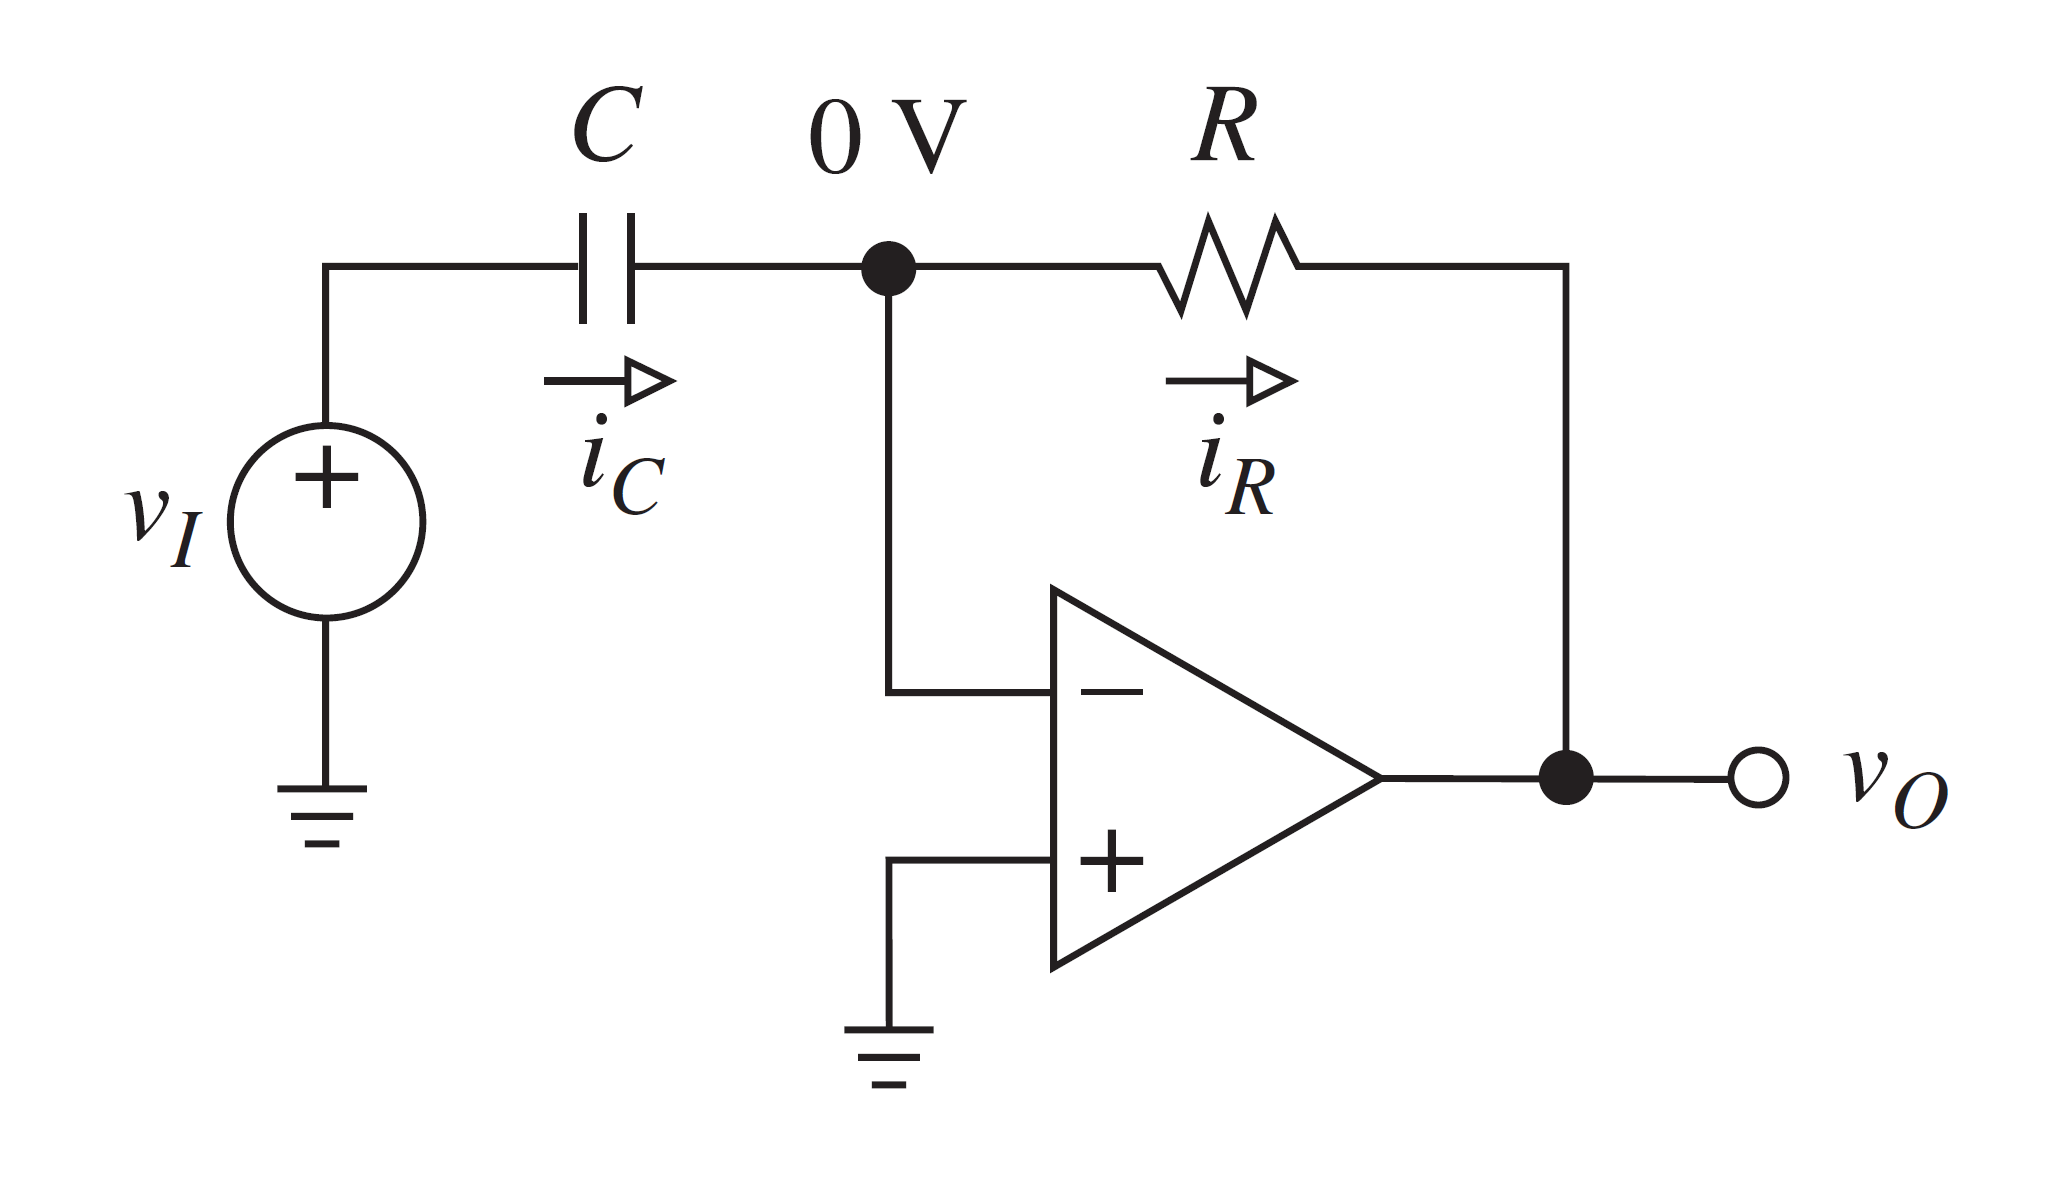
\includegraphics[scale=0.3]{1.3.6-Derivador.png}
\caption{amplificador derivador.}
\label{Fig:1.3.6.-Amplificador-Derivador}
\end{figure} 


\begin{figure}[h!] \centering
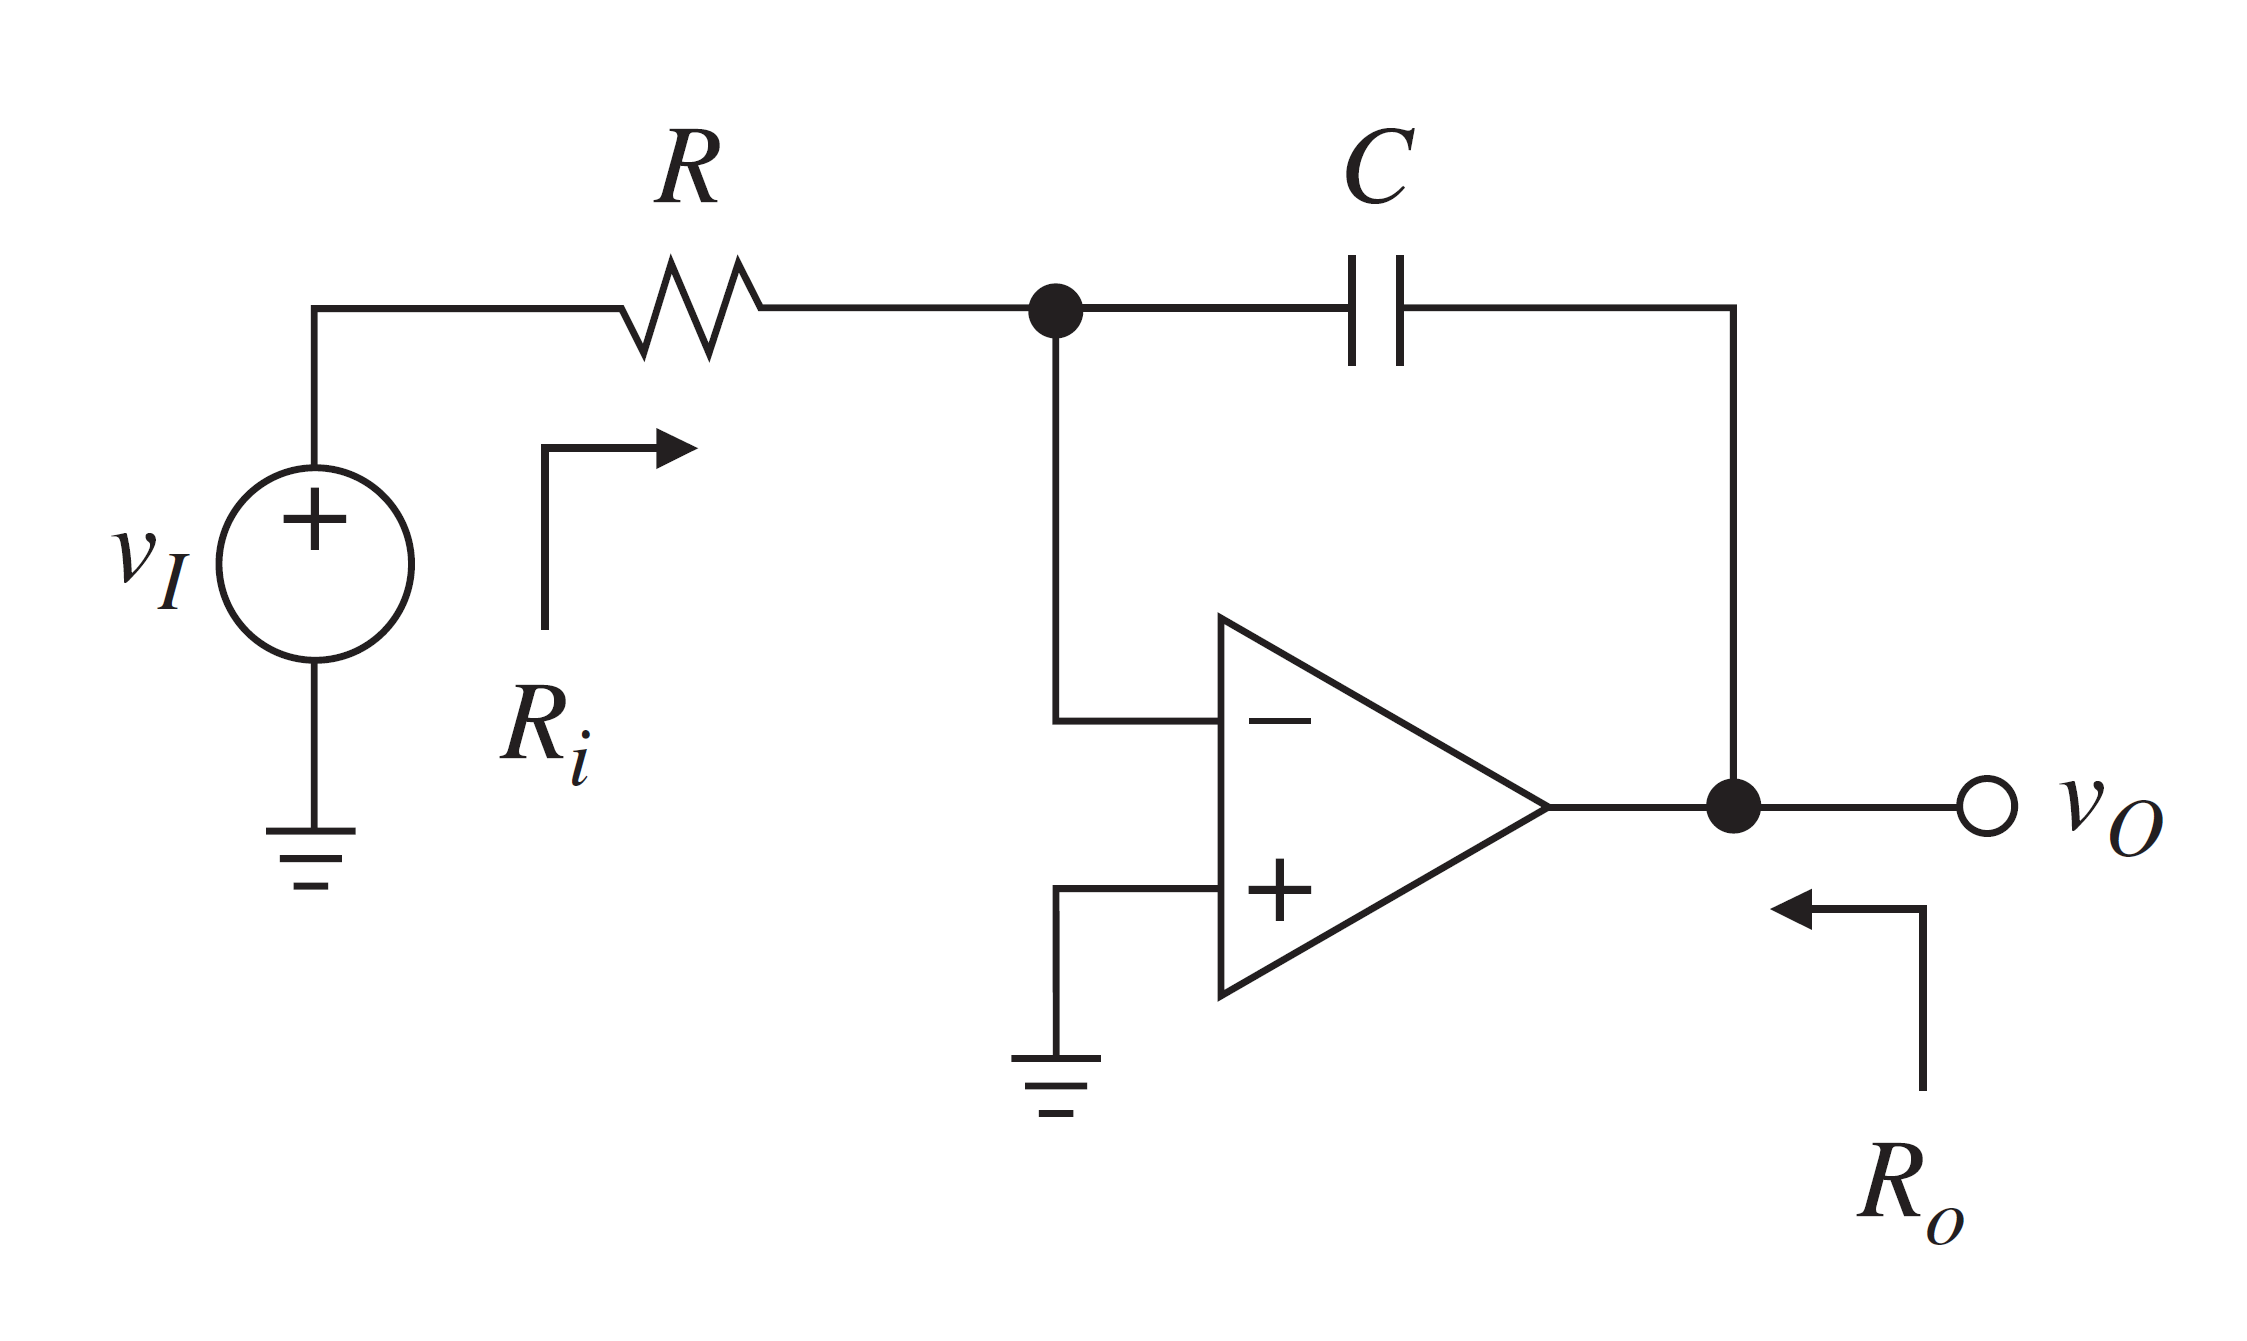
\includegraphics[scale=0.3]{1.3.7-Integrador.png}
\caption{amplificador integrador.}
\label{Fig:1.3.7-Amplificador-Integrador}
\end{figure} 


\newpage

\section{Filtrado}

Un filtro es un circuito que procesa señales dependientes de la frecuencia. La manera en que su comportamiento varía con la frecuencia se llama \textit{respuesta en frecuencia} y se expresa en términos de la \textit{función de trasferencia} $H(j\omega)$, donde $\omega = 2 \pi f$ es la \textit{frecuencia angular} y $j$ la unidad imaginaria ($j^2 = -1$). Esta respuesta se divide en dos: la \textit{respuesta de magnitud} $|H(\omega)$ y la \textit{respuesta de fase} $\measuredangle \ H(j \omega)$ que dan respectivamente la \textit{ganancia} y el \textit{cambio de fase} que experimenta una señala a través del circuito.

\subsection{Respuesta en frecuencia}

La función de trasferencia lo que hará es caracterizar la señal de salida y de entrada, y como se relaciona la fase/amplitud de dichas señales. Entonces la definimso como el cociente de la salida ($X_o$) y la entrada ($X_i$), tal que

\begin{equation}
H(j \omega) = \dfrac{X_o}{X_i}
\end{equation}
Como la respuesta en frecuencia de un circuito depende en gran medida de los elementos por los que este formado el mismo (condensadores,  bobibnas, resistencias). Sin embargo todos estes elementos tienen un factor en común: que ante una señal sinusoidal (señales con una sola frecuencia, como las que vamos a tratar) tienen un comportamiento lineal, ya que solo adelantan o retrasan la fase. Dado que las apariciones de $\omega$ llevan siempre un $j$ debido a los consdensadores/bobinas, podemos usar un término $s \equiv j \omega$ que generalice mejor el problema. En ese caso:

\begin{equation}
H(s) = \dfrac{N(s)}{D(s)} = \dfrac{a_m s^m + a{m-1} s^{m-1} + \cdots + a_1 s + a_0}{b_n s^n + a{n-1} s^{n-1} + \cdots + a_1 s + a_0}
\end{equation}
que son polinomios de $s$. Como todo polinomio complejo puede factorizarse (teorema fundamental del algebra), tenemos que puede expresarse como

\begin{equation}
H(s) = H_0 \dfrac{(s-z_1)(s-z_2)\cdots(s-z_m)}{(s-p_1)(s-p_2)\cdots (s-p_n)}
\end{equation}
donde $H_0 = a_m / bn$ se le llama \textit{factor de escalada}. Los términos de $z_i$ se llaman \textit{polos} y los términos $p_i$ se llaman polos. El grado del denominador determinará el \textit{orden} de la función de trasferencia. Las raíces (polos o ceros) de $N(s)$ y $D(s)$ son conocidos como \textit{frecuencias críticas} o \textit{frecuencias características}. Recordemos que las raíces pueden ser reales o complejas. 


\subsection{Filtros ideales}

Los \textit{filtros} son unos dispositivos que permiten pasar señales de ciertas frecuencias mientras otras frecuencias son rechazadas. La mayoría de los filtros se podrán modelizar como polinomios de manera muy efectiva, como veremos mas adelante. En general todos los filtros que creemos trataremos que se parezcan lo máximo posible a los filtros ideales. \\

Los filtros ideales son aquellos filtros que cumplen unas condiciones muy específicas: dejan pasar un rango muy determinado de frecuencias con una ganancia constante para cada una de estas; y luego matan al resto de frecuencias (tal que para estas $H=0$). En función del intervalo de frecuencias que pasan tenemos:

\begin{itemize}
\item El filtro a la \textbf{pasa-baja} solo deja pasar aquellas frecuencias inferior a la frecuencia de corte. Se puede ver en la figura \ref{Fig:2.03} a).
\item El filtro a la \textbf{pasa-alta} solo deja pasar aquellas frecuencias a partir de la frecuencia de corte. Se puede ver en la figura \ref{Fig:2.03} b).
\item El filtro a la \textbf{pasa-banda} solo deja pasar aquellas frecuencias dentro de un rango limitado por las frecuencias de corte. Se puede ver en la figura \ref{Fig:2.03} c).
\item El filtro a la \textbf{rechazo de banda} solo deja pasar aquellas frecuencias que están fuera de un rango limitado por las frecuencias de corte. Se puede ver en la figura \ref{Fig:2.03} d).
\end{itemize}

\begin{figure}[h!] \centering
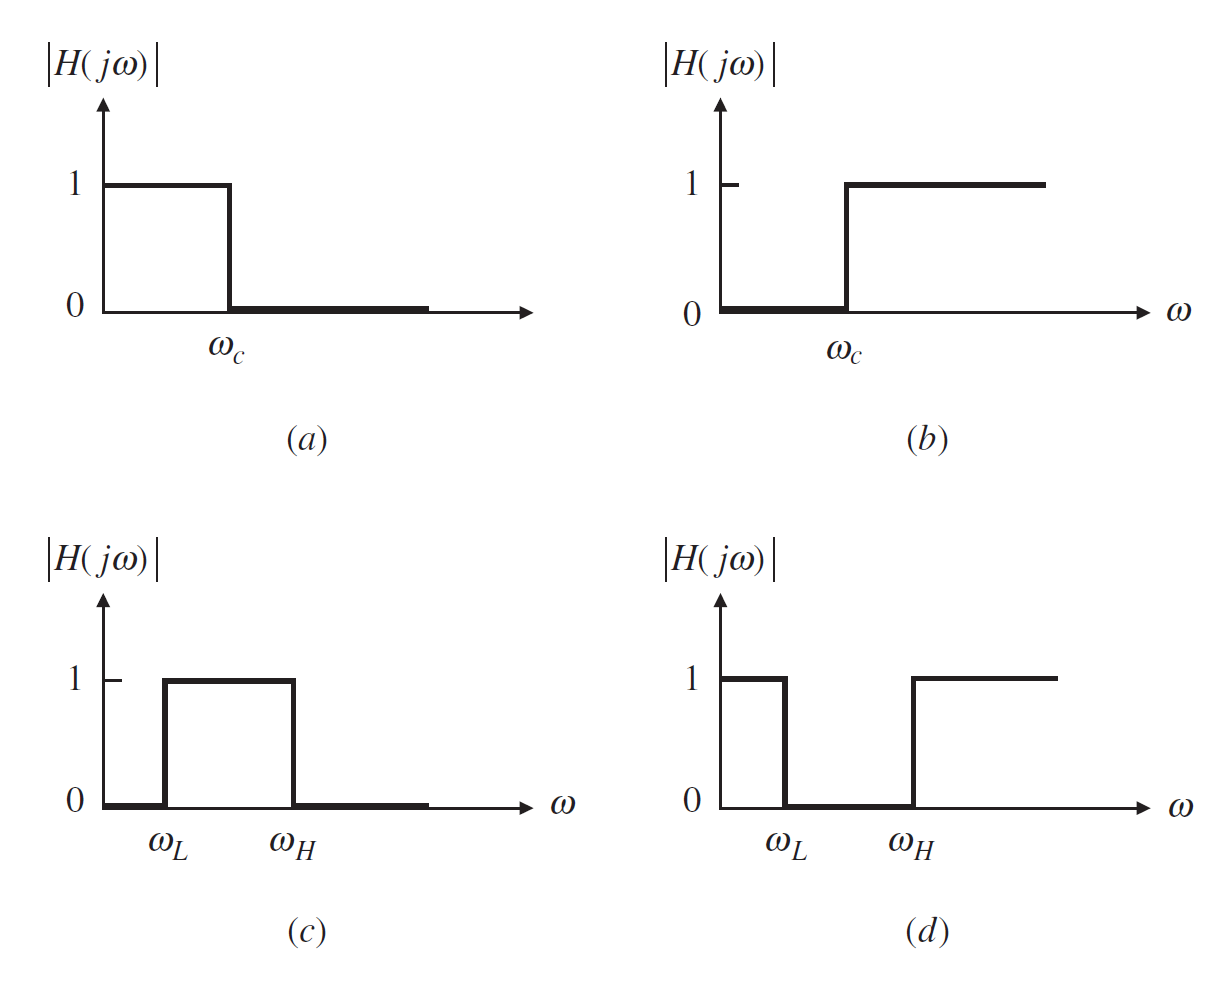
\includegraphics[scale=0.7]{2.2-Ideales.png}
\caption{Filtros ideales. Sergio Franco pag. 115.}
\label{Fig:2.03}
\end{figure}

\subsection{Filtros reales}

Por desgracia los filtros reales solo pueden aproximar los filtros ideales, de tal manera que cuanto mayor es el orden del filtro mas cercana será la aproximación que se desea. Cuando queremos representar la diferencia de un filtro real a uno ideal lo que hacemos es dibujar un área sombreado como podemos ver en las figuras \ref{Fig:2.04} y \ref{Fig:2.05}. \\ 

Para caracterizar los filtros creamos una serie de parámetros que nos permiten diferenciar las diferentes aproximaciones realizables. Llamamos al rango de frecuencias que pasan con poca o ninguna atenuación como \textit{banda de paso}. Para un filtro pasa-baja esta banda se extiende hasta la \textit{frecuencia de corte} $\omega_c$. Como vemos la ganancia en la banda de paso no tiene por qué ser constante, pudiendo exhibir rizos antes de la frecuencia . A la ganancia máxima $A_{\max}$ se le llama \textit{ganancia rizo en la banda de paso} y la banda de paso se denomina \textit{rizo de banda}. \\

Una vez se pasa de $\omega_c$ entramos en la \textit{banda de rechazo}. Esta banda se especifica en función de la la atenuación permisible, y viene determinada por $A_{\min}$. A la frecuencia a la que la banda de rechazo comienza se le llama $\omega_s$, y al factor $\omega_s / \omega_c$ se le llama \textit{factor de selectividad} porque brinda una medida de la nitidez de la respuesta. La región entre $\omega_c$ y $\omega_s$ se denomina \textit{banda de transición} o \textit{falda}. Esto se puede extender con facilidad los filtros pasa-alta, pasa-banda y rechaza-banda. \\


\begin{figure}[h!] \centering
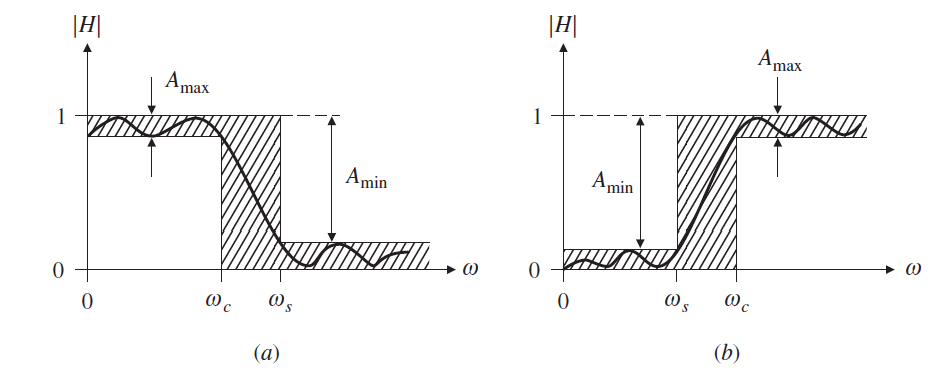
\includegraphics[scale=0.9]{2.2-Reales1.png}
\caption{Filtros pasa-baja y pasa-alta reales. Sergio Franco pag. 172.}
\label{Fig:2.04}
\end{figure}

\begin{figure}[h!] \centering
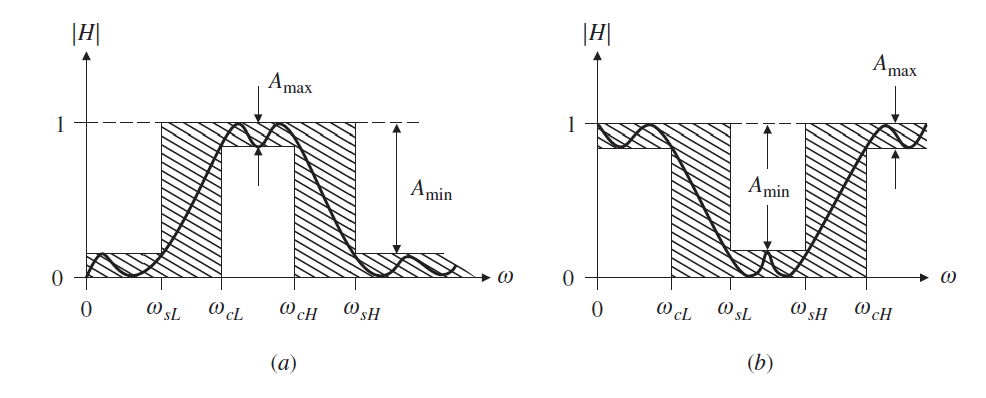
\includegraphics[scale=0.9]{2.2-Reales2.png}
\caption{Filtros pasa-banda y rechaza-banda reales. Sergio Franco pag. 173.}
\label{Fig:2.05}
\end{figure}


Como hemos dicho los filtros de mayor orden ($n$) permiten un mayor grando de optimización ya que constan de más coeficientes con los que poder aproximarse a los filtros ideales. Entre las diferentes aproximaciones existen varias muy satisfactorias, que optimizan ciertos rasgos. Estos son: \textit{Butterworth, Chebyshev, Bessel}. Véase figura \ref{Fig:2.06}. \\

\subsubsection{Filtro de Butterworth}

El filtro de Butterworth es un filtro con una ganancia que viene dada por:

\begin{equation}
|H(j \omega )| = \dfrac{1}{\sqrt{1+\epsilon^2 (\omega /  \omega_c)^{2n}}}
\end{equation}
donde $n$ es el orden del filtro, $\omega_c$ es la frecuencia de corte y $\epsilon$ es una constante que determina la variación máximo pasa banda $A_{\max}$.  Tiene como ventajas, frente a otros filtros, que su banda pasante es bastante plana, que su respuesta escalón es mucho mejor que el filtro de Chebyshev y una atenuación mayor que la de Bessel por encima de la banda pasante. Como desventaja tiene rizado en la respuesta a un escalón (una señal escalón). El orden del filtro nos dará el número de máximos/mínimos del rizado. Véase figura \ref{Fig:2.07}.

\subsubsection{Filtro de Chebyshev}

El filtro de Chebyshev consta de una ganancia que viene dada por:

\begin{equation}
|H(j\omega)| = \dfrac{1}{\sqrt{1+\epsilon^2 C_n^2 (\omega/\omega_c)}}
\end{equation}
donde $C_n(\omega/\omega_c)$ es un polinomio de Chebysehv de orden $n$, que se define como:

\begin{equation}
C_n (\omega/\omega_c) = \left\lbrace \begin{array}{cl}
\cos [n  \cdot \arccos (\omega/\omega_c)] & \ \ \mathrm{si} \ \omega/\omega_c \leq 1 \\ \\
\cosh [n \cdot  \arccosh (\omega/\omega_c)] & \ \ \mathrm{si} \ \omega/\omega_c \geq 1 
\end{array}  \right.
\end{equation}

Tiene como ventajas que da una mayor atenuación que la de Butterworth por encima de la banda pasante. Como claros inconvenientes tiene rizado en la banda pasante y una respuesta a un escalón (a una señal escalón) mucho peor que la de Butterworth. 

\subsubsection{Filtro de Bessel}

La ventaja mas grande del filtro de Bessel es que tiene la mejor respuesta a una señal escalón de los 3 filtros, aunque tiene una atenuación más lenta que Butterworth por encima de la banda pasante. 


\begin{figure}[h!] \centering
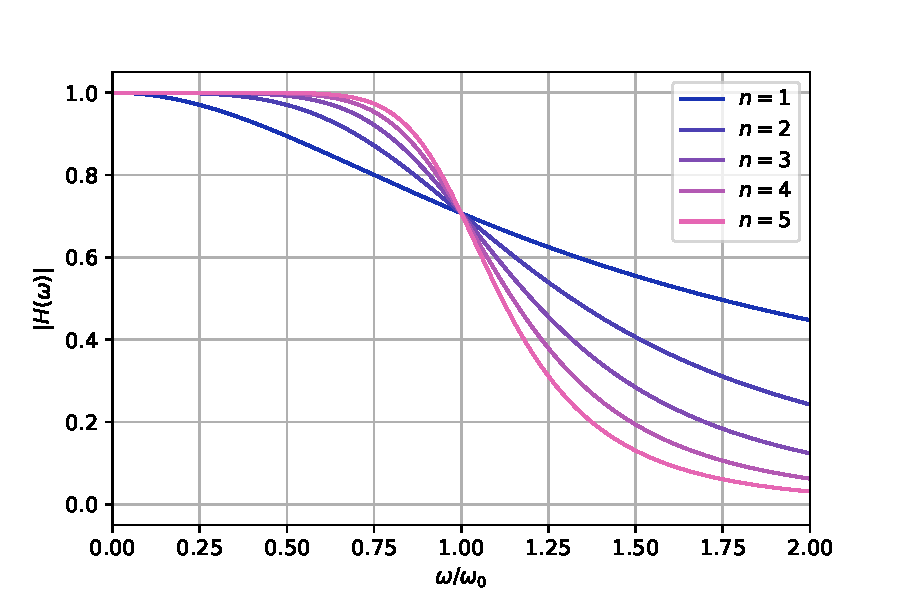
\includegraphics[scale=0.75]{2.3-Butterworth.pdf}
\caption{Filtros de Buttweworth pasa-baja para diferentes ordenes.}
\label{Fig:2.06}
\end{figure}

\begin{figure}[h!] \centering
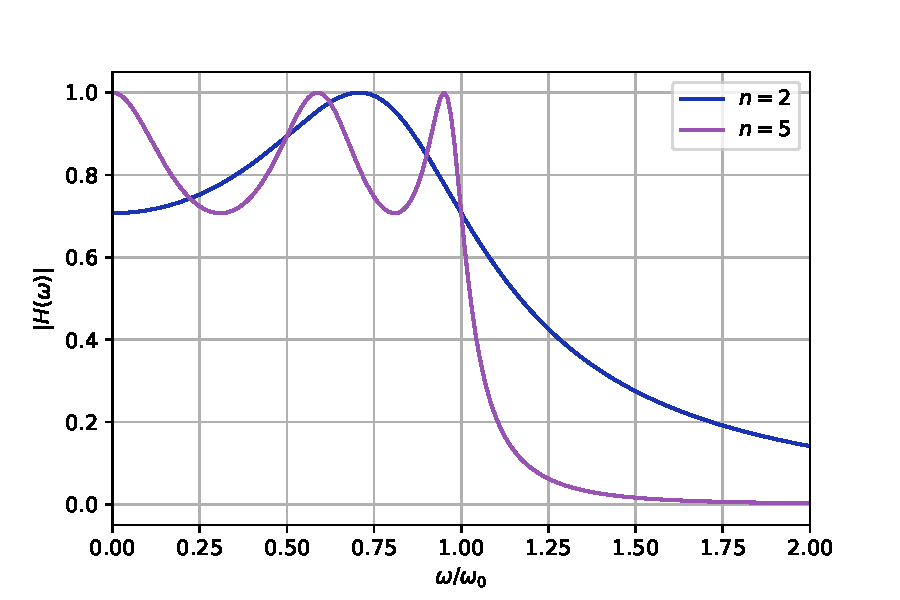
\includegraphics[scale=0.75]{2.3-Chebyshev.pdf}
\caption{Filtros de Chebyshev pasa-baja para diferentes ordenes.}
\label{Fig:2.07}
\end{figure}

\subsection{Filtrado con Amplificadores operacionales}

El diseño de un filtro es muy complejo, ya que primero tenemos que saber que tipo de filtro queremos hacer (pasa-baja, pasa-alta...), que modelo queremos usar (filtro de Butterworth...) y cuanto queremos que se parezca al filtro ideal (orden del filtro...). Además de esto tenemos que saber que elementos queremos usar: podemos construir un filtro pasivo (filtro RC, filtro RLC); o un filtro activo con amplificadores operacionales (Soluciones Sallen-Key...). En este tema veremos las soluciones más comunes. \\

\subsubsection{Solución Sallen-Key}

La \textit{solución Sallen-Key} también es llamada la \textit{solución KRC}. La topología usada será un circuito como el de la figura \ref{Fig:2.08} El amplificador operacional usado puede ser un circuito amplificador usando un A.O.I., ya que como hemos visto un circuito amplificador es, al final, un amplificador operacional con características controlables. Por ejemplo si usamos un seguidor de tensión (buffer) tendríamos que $K=1$, o si usamos una configuración no inversora $K=1+R_2/R_1$. Su función de trasferencia:

\begin{equation}
H(s) = \dfrac{K Y_1 Y_4}{Y_5(Y_1+Y_2+Y_3+Y_4) + Y_4(Y_1+(1-K)Y_2+Y_3)}
\end{equation}
De este modo tendremos un filtro u otro dependiendo de la elección de las amictancias. Recordemos que las amictancias vienen dadas por $I = Y \cdot V$, al contrario de las impedancias $Z$. 

\begin{figure}[h!] \centering
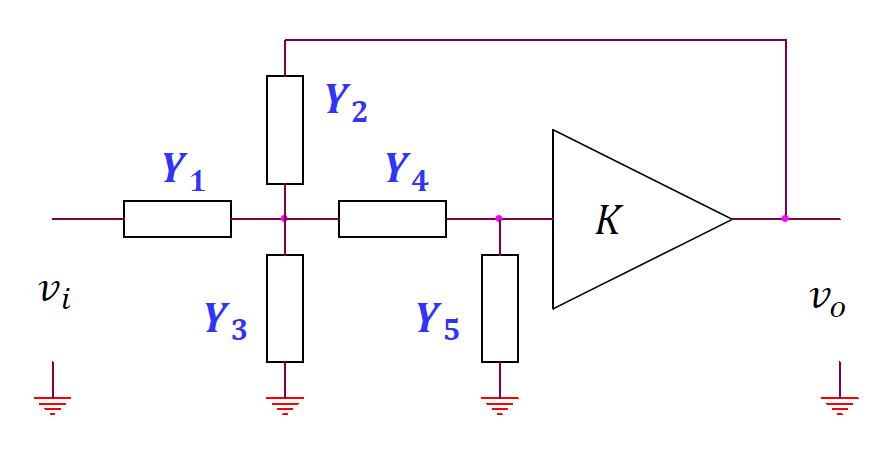
\includegraphics[scale=0.55]{2.4-KRC}
\caption{topología de la solución Sallen-Key.}
\label{Fig:2.19}
\end{figure}


\subsubsection{Solución MFB}

La \textit{solución MFB}, también llamada \textit{solución de retroalimentación múltiple} es uno de los filtros mas usados hoy en día (filtros de segunda orden). A diferencia de los filtros KRC; estos filtros aprovechan toda la ganancia de lazo abierto, y por eso a veces se llaman \textit{filtros de ganancia infinita}. 

\begin{figure}[h!] \centering
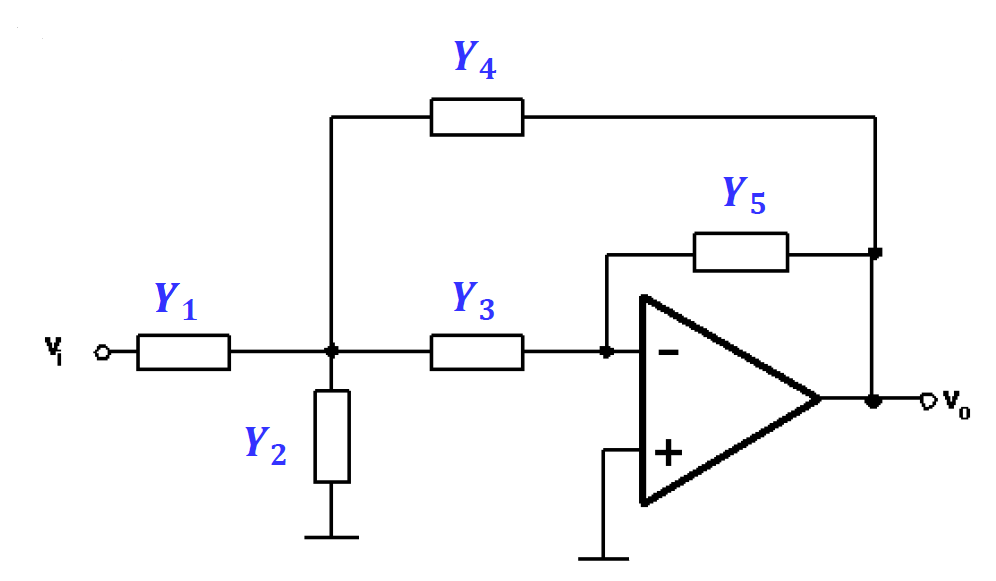
\includegraphics[scale=0.45]{2.4-MFB}
\caption{topología de la solución MFB.}
\label{Fig:2.20}
\end{figure}

\subsection{Clasificación de filtros}
\subsubsection{Filtros de primer orden}

Un filtro de primer orden puede ser un filtro pasa-baja (L.P.) o pasa-alta (H.P.). Dichos filtros tienen la siguiente forma:

\begin{equation}
L.P:  \ H(s) = \dfrac{a_0}{s+\omega_0} \tquad  
H.P:  \ H(s) = \dfrac{a_1 s}{s+\omega_0} 
\end{equation}

Al valor $\omega_0$ se le conoce como \textit{frecuencia de -3} dB ya que cuando $\omega=\omega_0$ tenemos que la frecuencia cae 3 dB respecto $H_0$ en la banda de paso; que sería $a_0/\omega_0$ o $a_1$ en función si el filtro es pasa baja o pasa alta, respectivamente. La banda de rechazo tendrá una caída de 20dB por década. La $\omega_1$ es el valor que verifica $H(j\omega_1)=0$ en un filtro a la pasa baja.

\begin{figure}[h!] \centering
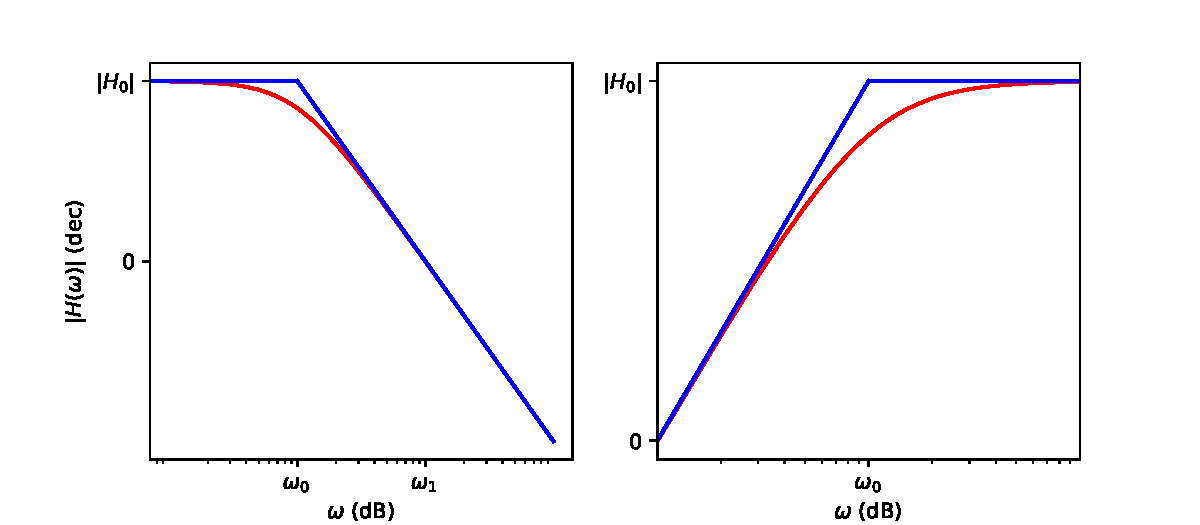
\includegraphics[scale=0.9]{2.4-1orden.pdf}
\caption{Filtros de primer orden pasa baja (izquierda) y pasa alta (derecha)}
\label{Fig:2.08}
\end{figure}

\subsubsection{Filtros de segundo orden}

Los filtros de segundo orden son mucho más generales, habiendo 6 tipos diferentes. Estos filtros son: pasa-baja (low-pass, LP), pasa-alta (high-pass, HP), pasa-banda (band-pass, BP), Notch, pasa-baja Notch (LPN), pasa-alta Notch (HPN).  En ese caso tenemos que:

\begin{equation}
L.P:  \ H(s) = \dfrac{a_0}{s^2 + \frac{\omega_0}{Q}s + \omega_0^2} \tquad  
H.P:  \ H(s) = \dfrac{a_2 s^2}{s^2+ \frac{\omega_0}{Q} s + \omega_0^2}  
\end{equation}
\begin{equation}
B.P:  \ H(s) = \dfrac{a_1 s}{s^2+ \frac{\omega_0}{Q} s + \omega_0^2} \tquad
Notch:  \ H(s) = \dfrac{a_2 (s^2 + \omega_0^2)}{s^2+ \frac{\omega_0}{Q}s + \omega_0^2}   
\end{equation}
\begin{equation}
L.P.N:  \ H(s) = \dfrac{a_2 (s^2 + \omega_n^2)}{s^2+\frac{\omega_0}{Q}s+ \omega_0^2}  \tquad
H.P.N:  \ H(s) = \dfrac{a_2 (s^2 + \omega_n^2)}{s^2+\frac{\omega_0}{Q}s+ \omega_0^2} 
\end{equation}
Como podemos ver LPN y HPN son exactamente iguales. La única diferencia es que LPN tiene que $\omega_n \geq \omega_0$ y que HPN que $\omega_n \leq \omega_0$. \\

Estas son las expresiones mas generales de los filtros de segundo orden, escritos en función de dos factores: \textit{la frecuencia natural de los polos} $\omega_0$ y \textit{el factor de calidad} $Q$.


\begin{figure}[h!] \centering
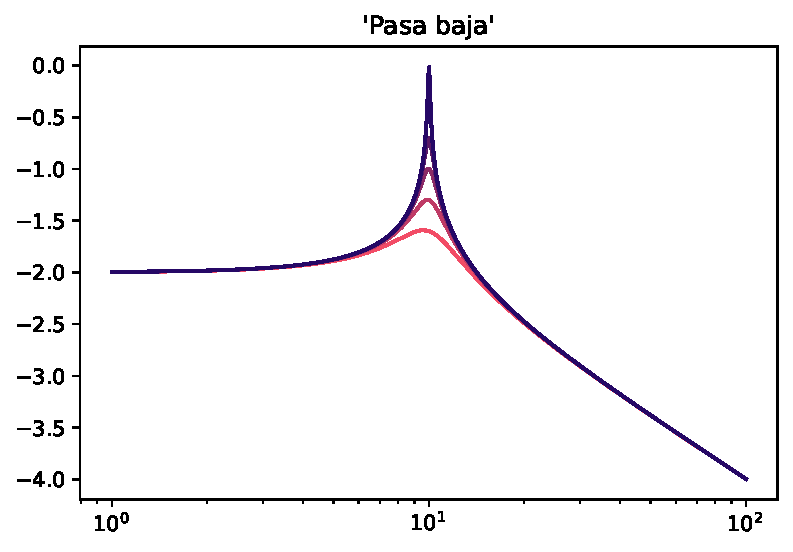
\includegraphics[scale=1.2]{Bode_1.pdf}
\end{figure}

\begin{figure}[h!] \centering
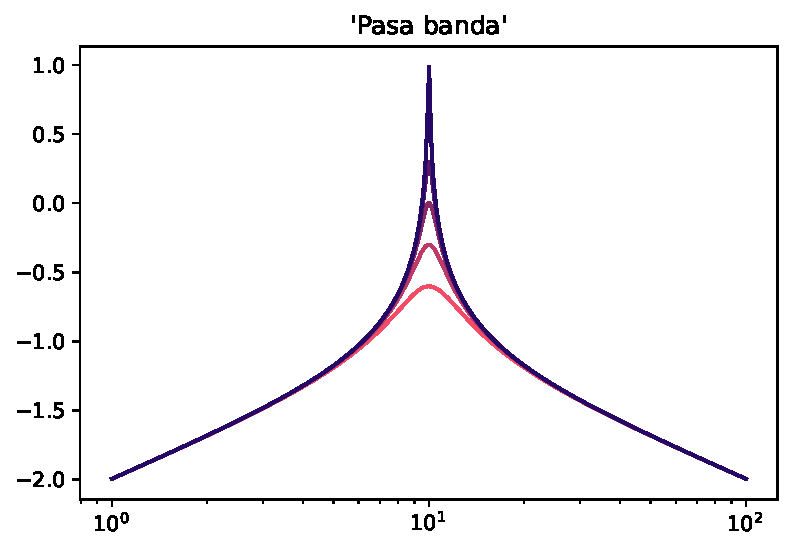
\includegraphics[scale=1.2]{Bode_2.pdf}
\end{figure}

\begin{figure}[h!] \centering
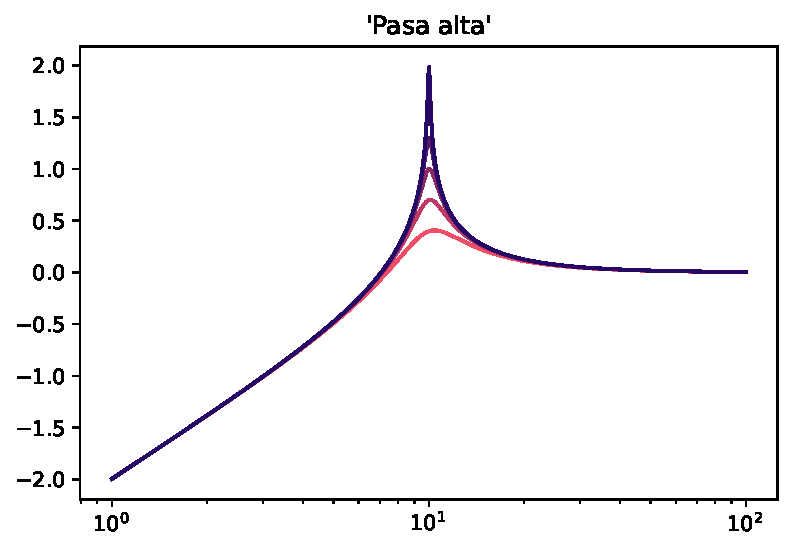
\includegraphics[scale=1.2]{Bode_3.pdf}
\end{figure}

\begin{figure}[h!] \centering
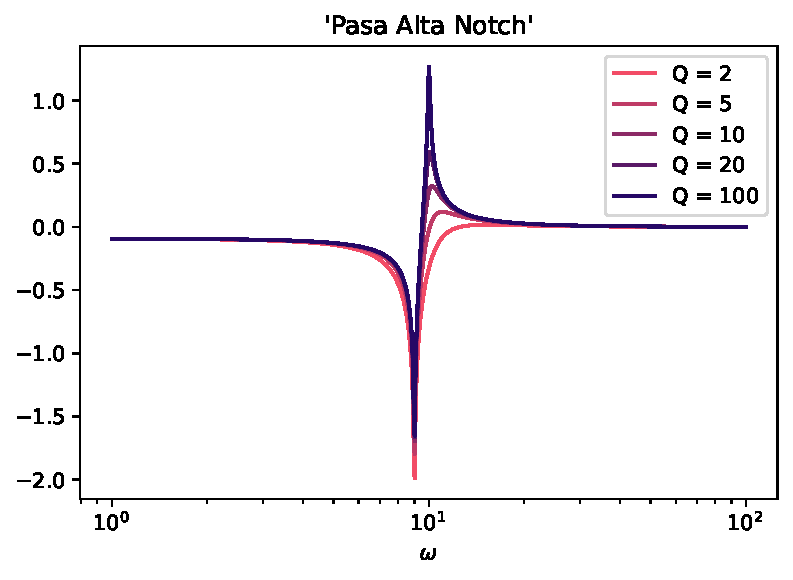
\includegraphics[scale=1.2]{Bode_4.pdf}
\end{figure}

\begin{figure}[h!] \centering
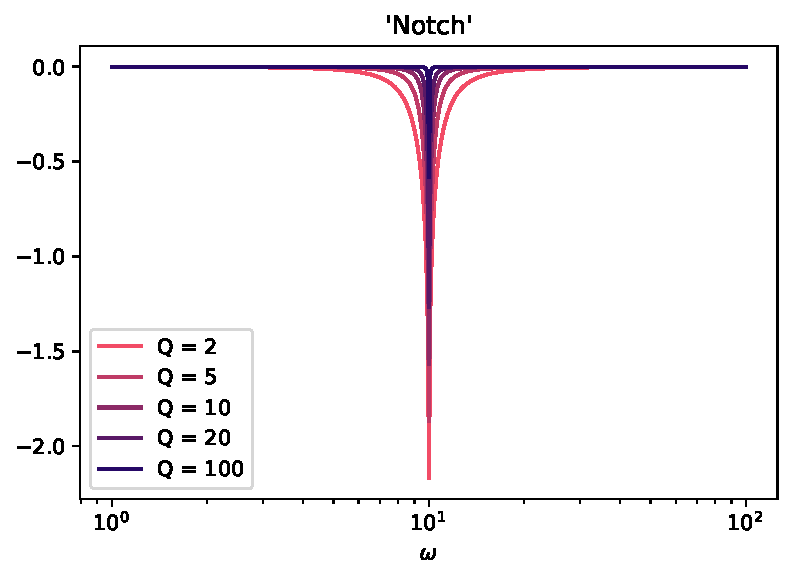
\includegraphics[scale=1.2]{Bode_5.pdf}
\end{figure}

\begin{figure}[h!] \centering
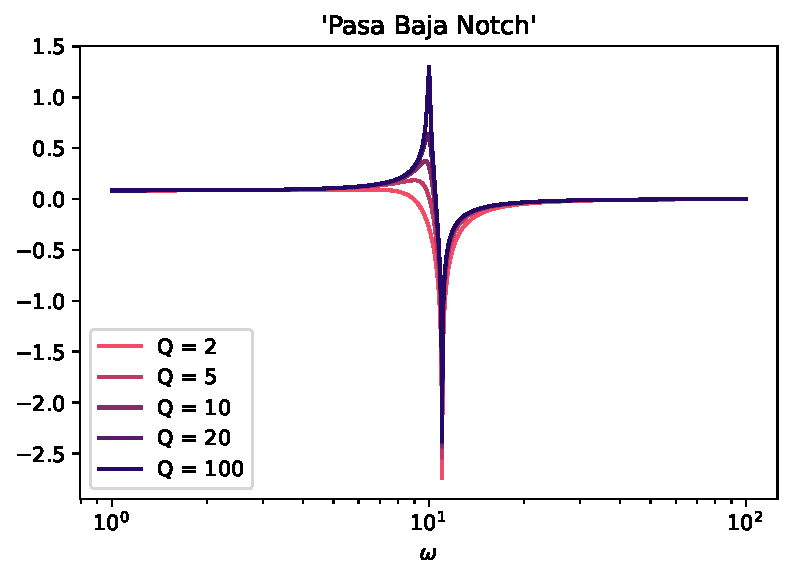
\includegraphics[scale=1.2]{Bode_6.pdf}
\end{figure}


\newpage

\section{Conversion de datos }

En su estado natural las variables portadoras de información se encuentran en forma analógica. Sin embargo, para propósitos de procesamiento, trasmisión y almacenamiento con frecuencia es más conveniente representar la información en forma digital. A su vez esto supone un problema, ya que crea la necesidad de convertir la información analógica a digital (convertidor A-D) y de digital a analógica (convertidor D-A). \\

%Si queremos sacar una señal en el rango 0V a 1V con una exactitud de 0.1mV del 0.1\%. Encontrar un amplificador operacional con estas características es difícil. Sin embargo podemos relajar las demandas del amplificador si lo que hacemos es expresar la información de manera digital. Esto se puede hacer representando el voltaje de salida con $v=0.d_1d_2d_3$<, con cada uno de los $d_i$ como un dígito decimal del 1 al 9. Si fuéramos capaces de convertir la señal de entrada en 3 dígitos decimales obtendríamos la misma información. Esto se puede hacer usando 3 circuitos, de tal modo que cada uno de ellos necesitaría resolver uno de los dígitos con una precisión aproximada del 5\%. Como podemos ver esto relajaría mucho la exigencia del problema. \\

%Sin embargo si somos capaces de crear 3 dígitos también tendremos que ser capaces de sintetizar esta información a través de un convertidor D-A de tal forma que $v=d_1 10^{-1} + d_2 10^{-1} + d_3 10^{-3}$. con una exactitud del 1 mV. \\

La representación mas eficiente es cuando los dígitos que usamos para representar la señal de entrada son 0 o 1. Cada uno de estos dígitos binarios los llamamos \textit{bits}. La cantidad de ellos es arbitraria, de tal modo que podamos tener 1,2,3 o 8 \textit{bits} para representar una señal. Una cadena de $n$ bits forman lo que se llama una \textit{palabra} de $n$ bits (que sería $b_1b_2b_3...b_n$). El bit $b_1$ representa el \textit{bit más significativo} (MSB) y el bit $b_n$ el \textit{bit menos significativo} (LSB). A la cantidad 

\begin{equation}
D = b_1 2^{-1} + b_2 2^{-2} + b_3 2^{-3} + \cdots + b_n 2^{-n}
\end{equation}
se le denomina \textit{valor binario fraccional}. Dependiendo del patrón del bit, $D$ puede asumir valores igualmente espaciados entre los valores $2^n$ hasta de $1-2^{-n}$. El límite inferior es alcanzado cuando todos los bits son iguales a cero y el superior cuando todos los bits son iguales a 1, y el espacio entre valores adyacentes es $2^{-n}$

\subsection{Convertidor D-A}

Un convertidor digital-analógico binario acepta una palabra de entrada de $n$ bits $b_1 b_2...b_n$ con un valor binario fraccional $D_I$ que produce una señal analógica proporcional a $D_I$. Entonces la señal de salida vendrá dada por:

\begin{equation}
v_O = K V_{\mathrm{REF}} D_I = V_\FSR (b_1 2^{-1} + b_2 2^{-2} + b_3 2^{-3} + \cdots + b_n 2^{-n})
\end{equation}
donde $K$ es un factor de escala y $V_\REF$ es un \textit{voltaje de referencia}. Al factor $V_\FSR \equiv K V_\REF$ se le llama \textit{rango de escala completa}. Aunque se suele usar la salida de voltaje también se puede usar la corriente como señal analógica, de manera completamente análoga. \\

De acuerdo con el patrón de entrada $v_O$ puede asumir $2^n$ diferentes valores, desde 0 hasta el \textit{valor de escala completa} $V_\FSV = (1-2^{-n}) V_\FSR$. Claramente la contribución de cada \textit{bit} al factor de escala completa es diferente. Por ejemplo la contribución del MSB es de $V_\FSR /2$, y la contribución del LSB es de $V_\FSR / 2^{n}$. Este último se le llama también \textit{resolución}. Se le llama así porque es la diferencia entre dos valores consecutivos.  En la imagen \ref{Fig:3.01} podemos ver como se comporta un convertidor D-A ideal de 3 bits.   \\

\begin{figure}[h!] \centering
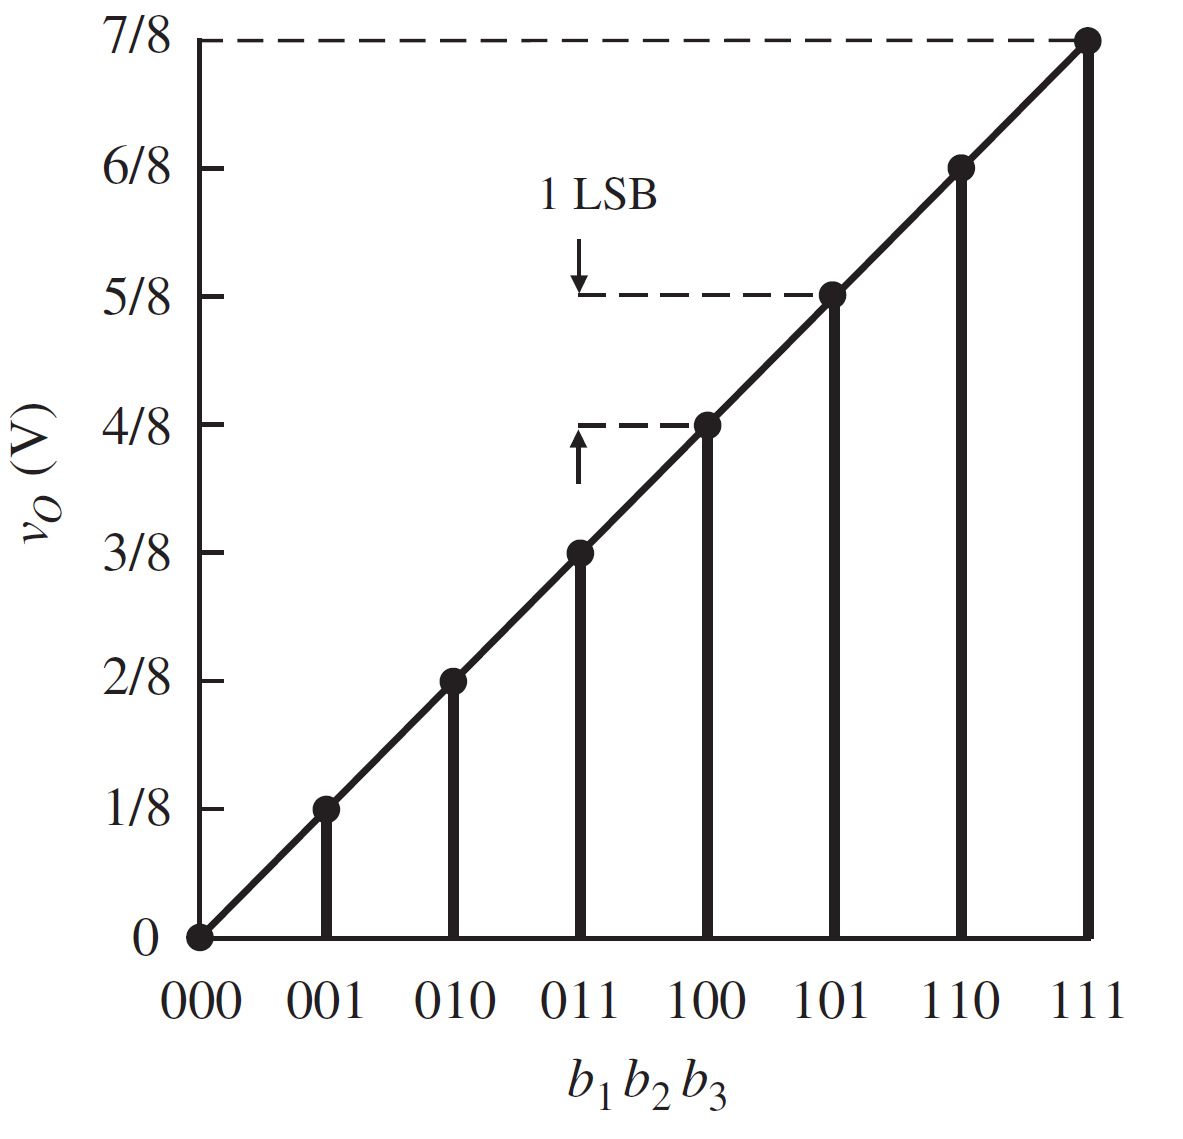
\includegraphics[scale=0.35]{3.1-Ideal.png}
\caption{convertidor D-A ideal con el factor de escala normalizado $V_\FSR = 1$.}
\label{Fig:3.01}
\end{figure} 

Sin embargo un sistema de circuitos internos de un convertidor digital-analógico está sujeto a error. Existen dos tipos de errores: los errores lineales y los errores no lineales. 

\subsubsection{Errores}

Los errores no lineales son dos: el \textit{error de desvío} o \textit{offset} y el \textit{error de ganancia} o \textit{gain}. Ambos errores son ajustables y corregibles con facilidad. \\

El \textbf{error de offset} es el error mas sencillo. Este tipo de error suma un voltaje a la palabra 0 (todos los bits son ceros). Normalmente se mide en LSB y se calcula como:

\begin{equation}
E_{off} = \left. \dfrac{V_o}{V_{\mathrm{LSB}}} \right|_{00 \ldots 0}
\end{equation}
es un error fácil de anular ya que solo habría que sumar a la salida un voltaje que anule el error. \\

El \textbf{error de ganancia} es un error que se puede eliminar ajustado el factor de escala $K$. Sabemos con precisión que el voltaje entre la palabra más grande (11...1) y la palabra mas pequeña (00...0) en el caso ideal es $(2^n-1)/V_\LSB$. Sin embargo puede ser que la distancia entre el valor mas pequeño y el mas grande no coincida con este valor. La diferencia entre el caso real e ideal sera el error de ganancia medido en LSB:

\begin{equation}
E_g = \parentesis{\left. \dfrac{V_o}{V_{\mathrm{LSB}}} \right|_{11 \ldots 1} - \left. \dfrac{V_o}{V_{\mathrm{LSB}}} \right|_{00 \ldots 0}} - (2^n-1)
\end{equation}

En la imagen \ref{Fig:3.02} se puede ver que claramente como son los errores. En la imagen de la derecha se ha corregido el error de offset para ver con mas claridad cual es el error de ganancia. \\

Los errores no lineales son dos: el \textit{error de no linealidad diferencial} (DNLE) y el \textit{error de no linealidad integral} (INLE). Estos errores se construyen a partir de los \textbf{valores compensados}. Llamamos valores compensados a aquellos valores a los que se le han corregido los errores de offsett y de ganancia. Entonces el valor compensado (en LSB) para la palabra número $i$:

\begin{equation}
\left. V_{comp}  \right|_i = V_o - E_{off} - \dfrac{i}{2^n - 2} E_g
\end{equation}
Una vez tenemos los valores compensados tendremos que los errores no lineales diferenciales y errores no integrales diferenciales.  Los errores no lineales es un array, un vector. Los \textbf{errores no lineales diferenciales} (DNLE) y \textbf{errores no lineales integrales} (INLE) son:

\begin{equation}
\DNLE_{j+1} = \dfrac{V_o|_{j+1} - V_o|_{j} - V_\LSB}{V_\LSB} \tquad 
\INLE_{j+1} = \dfrac{1}{V_\LSB} \sum_{i=0}^j \parentesis{ V_o|_{i+1} - V_o|_{i} - V_\LSB}
\end{equation}

\begin{figure}[h!] \centering
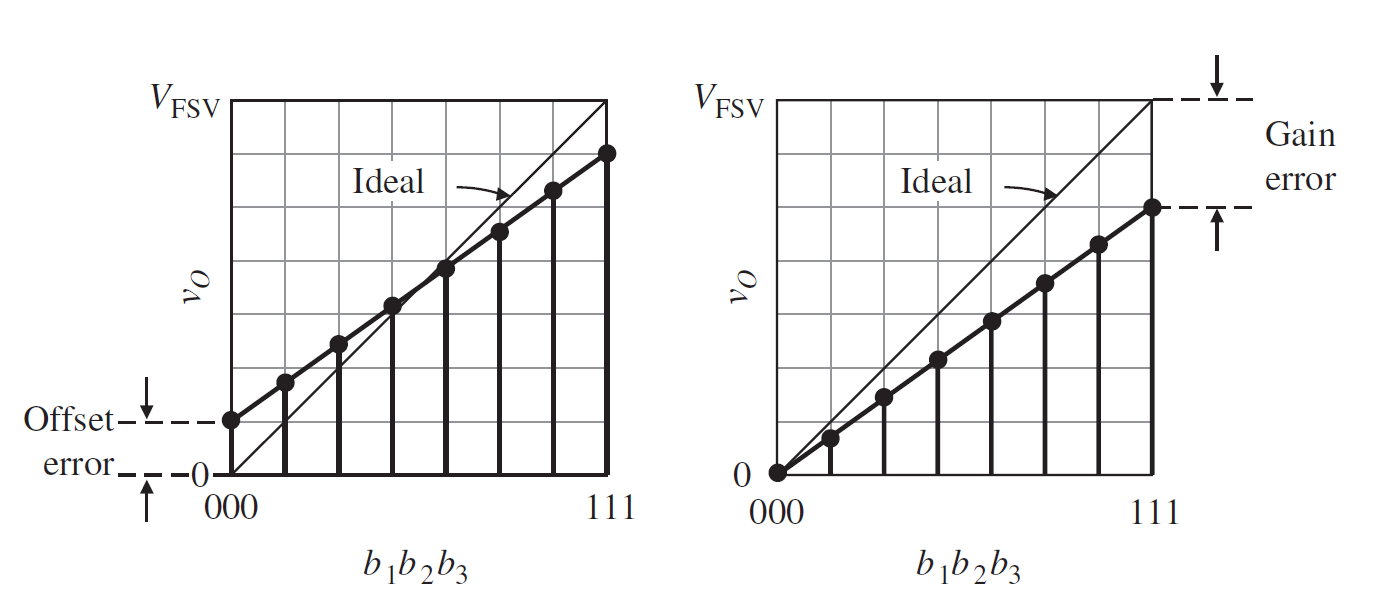
\includegraphics[scale=0.70]{3.1-Errores.png}
\caption{convertidor D-A con los errores lineales.}
\label{Fig:3.02}
\end{figure} 

\subsection{Convertidor A-D}

Un convertidor A-D lo que hace es leer una entrada analógica y la convierte en una palabra digital $b_1 b_2 \ldots b_n$. Entonces tenemos la entrada $v_I$ debe ser convertido en el valor fraccional $D_o$ tal que:

\begin{equation}
D_o = b_1 2^{-1} + b_2 2^{-2} + \cdots + b_n 2^{-n} = \dfrac{V_I}{K  V_\REF} = \dfrac{V_I}{V_\FSR} 
\end{equation}


 
 
\end{document}


